\newcommand{\ourmethod}{\text{DAIM}}
\newcommand{\policypi}{\mathbf{\pi} }
\newcommand{\expection}{\mathbb{E} }
\newcommand{\tables}{{Table }}
\newcommand{\eq}{{Equation }}
\newcommand{\alg}{{Algorithm }}
\newcommand{\starcraft}{{StarCraft II}}

\chapter{Diversity-Augmented Intrinsic Motivation}
\label{ch:daim}
\section{Introduction}
In order to improve sample efficiency of DRL algorithms in the environments offering sparse rewards, Chapter~\ref{ch:esil} proposes a novel self-imitation loss function to increase the frequency that the agent achieves positive samples, and Chapter~\ref{ch:dtgsh} uses the determinantal point processes (DPPs) framework to measure the diversity of achieved goals in a trajectory and proposes a sampling strategy that uses diversity as a priority to sample the trajectories for further processing, in which diversity can also quantify the contribution of each trajectory. In this chapter, we keep exploring the potential application of determinantal point processes (DPPs) in deep reinforcement learning (DRL). In contrast to previous chapters, DPPs are used to quantify the discrepancy between adjacent states as additional endogenous rewards to accelerate the training of DRL agents in the environment with the sparse reward setting.

%Deep reinforcement learning (RL) allows agents to learn a wide range of reward-driven skills, including playing games~\cite{mnih2015human,silver2016mastering,xu2020neurips}, controlling robots~\cite{dai2020episodic,fang2018dher,gu2017deep,levine2016end}, and making decisions in other environments~\cite{fang2017learning,vinyals2017starcraft}. 

%Many significant application problems in DRL can be formulated as a 
% Many important applied problems in DRL can be accurately modelled as learning from extrinsic rewards, where a function (approximately) relates features associated with a state/action pair and the expectation of the resulting rewards. Furthermore, with appropriate features, it is often the case that linear or nonlinear functions can accurately approximate the reward function. However, hand-crafted reward functions usually lead to unexpected behaviors~\cite{riedmiller2018learning} and limited exploration. 
% Potential-based reward shaping methods~\cite{ng1999policy} offers a general answer to what degree of reward function modifications do not affect the optimal policy. Other works have tried to design auxiliary rewards to derive policies with desired properties. For example, Jaderberg \textit{et al.}~\cite{jaderberg2016reinforcement} calculate a pseudo-reward from unsupervised auxiliary tasks, and use this reward to refine its internal representation. In count-based methods~\cite{bellemare2016unifying, ostrovski2017count, tang2017exploration}, a pseudo-count based reward is used to encourage the agent to explore novel states in the environment.

% In environments or tasks for which the reward sparsity is higher, undirected, or even deceptive, the application of RL techniques is significantly more difficult, since the agent might have only occasional opportunities to improve its policy, such as when the final goal is reached. In such scenarios, agents can be endowed with mechanisms of {\it intrinsic motivation} that encourage exploration in environments and learn useful policies even without explicit supervision. Early attempts to incorporate intrinsic motivation use self-supervised prediction errors as intrinsic rewards to help the agent explore~\cite{pathak2017curiosity}. More recently, Zheng \textit{et al.}~\cite{zheng2018learning} design an augmented agent with additive intrinsic rewards. When the intrinsic value of the action is added to the task-dependent (i.e., extrinsic) rewards, the performance of policy gradient based learning methods can be improved. 
%Another line of work uses auxiliary control tasks, such as pixel control or feature control, which can significantly speed up learning of the main task. The rationale is that learning the auxiliary tasks gives the agent features that are useful for manipulating the environment. However, these intrinsic methods are either difficult to explain or only specific to some tasks.

Encouraging the agent to explore previously unseen/novel states in the environments with sparse or delayed reward settings is still a challenge in DRL. In this chapter, we demonstrate how a simple generated intrinsic reward function based on a diversity measure can enable RL agents to explore novel states efficiently. This generated auxiliary reward is functional for a number of environments, as confirmed by a selection of MuJoCo locomotion tasks and video games.

% Encouraging effective exploration of novel states for agents without any reward signal is still a challenging problem. Making progress on this problem requires specifying a learning objective that ensures the agent explores large parts of the state space. In this chapter, we demonstrate how a simple generated intrinsic reward function based on a diversity measure can enable RL agents to explore novel states efficiently. This auxiliary reward is functional for a number of environments, as confirmed by a selection of MuJoCo locomotion tasks and video games.

%We hypothesise that in order to acquire an agent that is useful and efficient, we must train the agent so that it can attain coverage over the set of possible states.

In order to obtain an agent that can solve the tasks with sparse or delayed rewards, we need the agent to explore as many novel states as possible during training. However, common exploration strategies ({e.g.}, random sampling, $\epsilon$-greedy) can re-visit previously explored states in the environment, which can limit the effectiveness of state-space coverage.

A key idea in our work is to use a measure of discrepancy between states as an intrinsic motivation. To model the diversity of the agent's states, we adopt the framework of determinantal point processes (DPPs)~\cite{kulesza2012determinantal} to formulate the intrinsic reward as a dynamic measure of diversity. Regarding the sequence of states as a DPP allows a measure of the diversity of subset selection, widely used in data summarization for selecting a diversified subset~\cite{gong2014diverse}. We build an intrinsic reward for diversity with parameterised DPPs and propose a new general method for learning policies with intrinsic rewards. The proposed method is referred to as diversity-augmented intrinsic motivation ($\ourmethod$). Through a series of experiments, we show that the agents trained with the proposed diversity-based intrinsic rewards learn effectively and attain higher rewards than well-known baselines, especially in continuous control environments.

The contributions of this chapter can be summarized as follows: 1) The DPPs framework is proposed as a measure for the diversity of adjacent states, and this diversity is used as the intrinsic reward, 2) A bi-level optimisation~\cite{zheng2018learning} is borrowed to combine with the proposed diversity-based measure, so that the intrinsic reward will increase the extrinsic reward while increasing diversity, and 3) $\ourmethod$ is evaluated in the MuJoCo locomotion and arcade learning environments. Empirical results demonstrate that $\ourmethod$ can outperform baseline methods in most of the standard tasks and outperform baselines in 12 out of 15 tasks with delayed rewards in the MuJoCo locomotion environment. In addition, $\ourmethod$ also improves the rate of learning in the initial stage of training in the arcade learning environment.
\newpage

\section{Related Work}
Intrinsic motivation is an approach to explore novel states which may lead to higher rewards in the future. Pathak \textit{et al.}~\cite{pathak2017curiosity} propose an intrinsic curiosity module (ICM), suggesting the prediction error between an actual encoded frame and the predicted encoded frame as the intrinsic reward. A higher prediction error indicates the agent has moved into a novel state, and this intrinsic reward will encourage the agent to keep exploring such novel states. In order to find an appropriate representation of pixels that could be invariant to insignificant changes in the environment, an inverse dynamic model is introduced to extract features. This requires training a network, which uses consecutive frames as input to predict the action that would transition the previous frame to the subsequent. The insight of the inverse dynamic model is that through predicting environment dynamics, features are learned to preserve the key information that predicts the action. Burda \textit{et al.}~\cite{burda2018largescale} conduct a large-scale study of curiosity-driven learning. Their findings suggest that an agent can learn to play a significant number of Atari games, even without receiving any extrinsic rewards from the environment. 

However, environments with stochastic dynamics may not be suitable for the application of purely exploratory approaches. Variational Information Maximising Exploration (VIME)~\cite{NIPS2016_abd81528} formulates the intrinsic reward based on the information gain according to the agent’s belief of environment dynamics, and it shows significant improvements in the continuous control tasks with the sparse reward setting. 

Zheng \textit{et al.}~\cite{zheng2018learning} introduce learning intrinsic reward for policy gradient (LIRPG), which enables a learnable intrinsic reward function to be used for training an RL agent. In addition, LIRPG adopts a bi-level optimisation scheme that when the policy network is updated to maximise the accumulated intrinsic and extrinsic rewards, the intrinsic reward function is also updated to maximise the accumulated extrinsic rewards achieved by the policy network. This optimisation scheme guarantees the learned reward function can generate meaningful intrinsic rewards to facilitate the agent reaching the ultimate goal (i.e., maximising the accumulated extrinsic rewards). In this work, we also leverage this bi-level optimisation to ensure the agent can explore novel states that deliver more accumulated extrinsic rewards.

\section{Methodology}
% start
\begin{figure}[t]
    \centering
    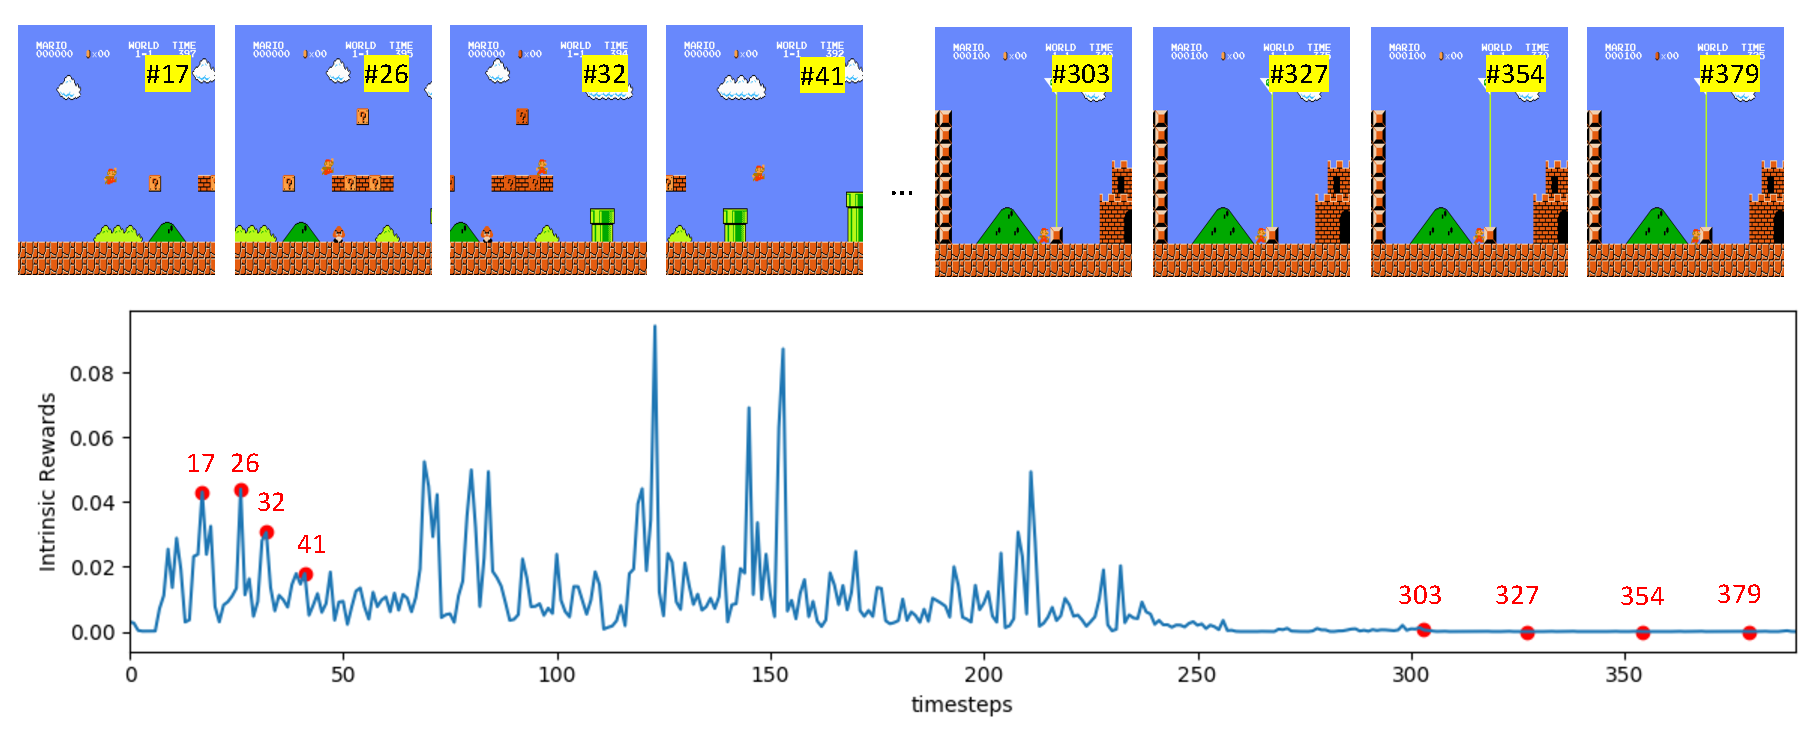
\includegraphics[width=\linewidth]{figures/chapter5/illustration.pdf}
    \caption[Illustration of $\ourmethod$.]{Illustration of $\ourmethod$. It shows the intrinsic rewards of an entire episode of SuperMarioBros. The red points annotate the key frames in the game. In frames \{17, 26, 32, 41\}, the agent keeps moving forward, and the intrinsic rewards are relatively higher. In the frames \{303, 327, 354, 379\}, the agent is stuck at the bottom of the flagpole. For these latter four frames, the diversity between adjacent states is very small, and the intrinsic rewards are close to zero.}
    \label{fig:illustration}
\end{figure}

In the proposed method, let $r_{t}^{\text{ex}}$ denote the extrinsic reward received from the environment and $r^{\text{in}}_{t}$ denote the intrinsic reward parameterised by $\eta$. The agent can receive a mixed reward represented in the following form:
\begin{equation}
    r^{\text{mix}}_t = \lambda^{\text{ex}} r^{\text{ex}}(s_{t}, a_t) + \lambda^{\text{in}} r^{\text{in}}(s_t, s_{t+1};\eta),
\end{equation}
where $\lambda^{\text{ex}}$ and $\lambda^{\text{in}}$ are the weight coefficients of the extrinsic reward $r^{\text{ex}}_{t}$ and the intrinsic reward $r^{\text{in}}_{t}$ at timestep $t$. The agent is updated to maximise the diversity-augmented return $G^{\text{mix}}(s_t,a_t)$, where $G^{\text{mix}}(s_t,a_t) =\sum_{k=0}^{T-1}\gamma^{k}r^{\text{mix}}_{t+k}$. Notice that the ultimate goal of the agent is still maximising the extrinsic return $G^{\text{ex}}(s_{t}, a_{t})$. 

In the rest of this section, we first introduce the primary objective function and the optimisation algorithm that can ensure the maximisation of the extrinsic return while increasing the diversity-augmented returns. Subsequently, the intrinsic reward formulated under the DPPs framework is discussed.

\subsection{Primary Objective Function}
To make sure that $\ourmethod$ still increases the extrinsic reward, we adopt a bi-level optimisation framework. The objective function is defined as follows:
\begin{align}
  \label{eq:obj}
  \max_{\eta}\quad & J^{\text{ex}}(\eta;\theta^{\prime}),\\ 
  \text{subject to}\quad & \theta^{\prime} =\mathop{\arg\max}_{\theta}\ J^{\text{mix}}(\theta, \eta).
  \nonumber
\end{align}
Here $J^{\text{mix}} = \mathbb{E}_{\pi_{\theta}}\bigr[G^{\text{mix}}(s_t,a_t) \bigr]$, and $\theta$ represents the parameters of the policy network.
The optimisation problem of \eqref{eq:obj} can be viewed as a bi-level optimisation, which is widely used in the fields of machine learning, such as meta-learning~\cite{andrychowicz2016learning,nichol2018first,santoro2016meta,xu2018meta,zheng2018learning}, signal processing~\cite{kunapuli2008classification,flamary2014learning}, and hyperparameters optimisation~\cite{franceschi2018bilevel, shaban2019truncated}. In Equation~\eqref{eq:obj}, $J^{\text{ex}}$ and $J^{\text{mix}}$ are upper-level and lower-level objective functions, respectively. The primary goal of this bi-level objective function is to maximise extrinsic returns (upper-level objective function) $J^{\text{ex}}$ with respect to the parameters of intrinsic reward $\eta$, and the updated parameters of the policy network $\theta^{\prime}$ can be achieved via maximising the lower-level objective function.

% The upper-level optimisation is treated as the leader, while the lower-level optimisation is the follower. The upper agent reshapes the reward to make the low-level agent's learning easier. The low-level agent observes the commands of the upper-level agent and works towards meeting the commands.

The policy parameters $\theta$ and the intrinsic parameters $\eta$ can be updated alternately.
Firstly, the update of the policy network $\pi_{\theta}$ with a learning rate $\alpha$ can be written as:
\begin{equation}
    \theta^{\prime}=\theta + \alpha\nabla_{\theta} \log \pi(a_t|s_t;\theta)G^{\text{mix}}(s_t, a_t).
\label{eq:mix_cost}
\end{equation}
Secondly, we update $\eta$ towards maximising the expected extrinsic returns $G^{\text{ex}}(s_t, a_t)$ of the agent. 
To build the connection between $J^{\text{ex}}$ and $\eta$, the updated parameters of the policy network $\theta^{\prime}$ are used to sample a new trajectory and solve the following problem:
\begin{equation}
    \max_{\eta} J^{\text{ex}} = \mathbb{E}_{\pi_{\theta^{\prime}|\eta}}[G^{\text{ex}}(s_t, a_t)].
\label{eq:cost_ex}
\end{equation}
Then, the gradient $\nabla_{\eta} J^{\text{ex}}$ can be calculated using the chain rule:
\begin{equation}
    \nabla_{\eta} J^{\text{ex}} = \nabla_{\theta^{\prime}}J^{\text{ex}}\nabla_{\eta}\theta^{\prime}, 
  \label{eq:chain_rule}
\end{equation}
with 
\begin{align}
    \nabla_{\eta}\theta^{\prime} &=  \nabla_{\eta}\alpha G^{\text{mix}}(s_t, a_t) \nabla_{\theta} \log \pi(a_t|s_t;\theta) \nonumber \\
    &= \alpha\lambda^{\text{in}}\sum_{k=0}^{\infty}\gamma^{k}\nabla_{\eta}r^{\text{in}}_{\eta,t+k}\nabla_{\theta} \log \pi(a_t|s_t;\theta). 
\end{align}

Here, instead of collecting another set of samples, importance sampling is employed to increase the sample efficiency of the algorithm:
\begin{equation}
    \nabla_{\theta^{\prime}}J^{\text{ex}} =  \nabla_{\theta^{\prime}}\Bigg (\frac{\pi(a_{t}|s_{t};\theta^{\prime})}{\pi(a_{t}|s_{t};\theta)}\Bigg ) G^{\text{ex}}(s_{t}, a_{t}).
\label{eq:importance_sampling}
\end{equation}
% The principle of the \eq \eqref{eq:chain_rule} is to formulate the effect of the change of $\eta$ on influencing $J^{\text{ex}}$ through its influence on the updated policy parameter $\theta'$.
%This is a commonly adopted technique in meta-gradient learning~\cite{andrychowicz2016learning,nichol2018first,santoro2016meta,xu2018meta,zheng2018learning}. 
Through this bi-level optimisation, the features that are learned ensure that the resulting diversity also increases the extrinsic returns. Furthermore, the value network is updated via a mean squared error loss $\mathcal{L}_{value} = \mathbb{E}[(V(s_{t};\psi) - G_{t}^{\text{mix}})^2]$. Algorithm~\ref{algo:vi} gives the pseudo code for our method -- diversity-augmented intrinsic motivation ($\ourmethod$). The code is publicly available at: \url{https://github.com/TianhongDai/daim-rl}.

\begin{algorithm}[t]
	\caption{\label{alg:all} Diversity-Augmented Intrinsic Motivation.
	}
	\begin{algorithmic}[1]
		\REQUIRE a policy network $\pi(a_{t}|s_{t};\theta)$, an intrinsic reward module $\phi(s_{t},s_{t+1};\eta)$, a value network $V(s_{t};\psi)$, learning rate $\alpha$, intrinsic module learning rate $\beta$, transition buffer $\mathcal{B}$, number of iterations $N$, length of each rollout $T$, weight coefficient of extrinsic reward $\lambda^{\text{ex}}$, weight coefficient of intrinsic reward $\lambda^{\text{in}}$
		%\STATE \textbf{Init}: initialize the policy network $\pi(a_{t}|s_{t};\theta)$ and intrinsic network $\phi(s_{t};\eta)$
		\FOR{iteration = 1, 2, 3, ..., $N$}
		\STATE Let $\mathcal{B} \leftarrow \varnothing$
		\FOR{$t$ = 1, 2, 3, ..., $T$}
        \STATE Sample an action $a_{t}$ using policy network $\pi(a_{t}|s_{t};\theta)$
        \STATE Execute the action $a_{t}$ and get the next state $s_{t+1}$ and the extrinsic reward $r^{\text{ex}}_{t}$
		\STATE Calculate the kernel matrix: $\textbf{L}_{y}=\mathbf{M}^{T}\mathbf{M}$ using $\phi(s_{t},s_{t+1};\eta)$
		\STATE Compute the intrinsic reward: $r_{t}^{\text{in}} = \det\left(\mathbf{L}_{y} \odot \left(\diag{(\mathbf{L}_{y}})^{T}\diag({\mathbf{L}_{y}})\right)^{-\frac{1}{2}}\right)$
		\STATE Store the transition $(s_{t}, r^{\text{in}}_{t}, r^{\text{ex}}_{t}, s_{t+1}, a_{t})$ in $\mathcal{B}$
		\ENDFOR
		\STATE Compute the diversity-augmented return $G^{\text{mix}}(s, a)$ using the mixed reward: $r^{\text{mix}}=\lambda^{\text{ex}}r^{\text{ex}} + \lambda^{\text{in}}r^{\text{in}}$
		\STATE Compute the extrinsic return $G^{\text{ex}}(s, a)$ using the extrinsic reward: $r^{\text{ex}}$
		\STATE Update $\theta$ according to Eq.\eqref{eq:mix_cost} with learning rate $\alpha$
		\STATE Update $\psi$ according to $\mathcal{L}_{value}=\mathbb{E}[(V(s_{t};\psi)-G^{\text{mix}}_{t})^2]$ with learning rate $\alpha$
		\STATE Update $\eta$ according to Eq.\eqref{eq:chain_rule} and Eq.\eqref{eq:importance_sampling} with learning rate $\beta$
        \ENDFOR
	\end{algorithmic}
	\label{algo:vi}
\end{algorithm}
\subsection{Parameterised Diversity as Intrinsic Reward}
We are now able to parameterise the intrinsic reward with parameter $\eta$ in this section. The intrinsic reward at timestep $t$ is defined as:
\begin{equation}
    r^{\text{in}}(s_t, s_{t+1}; \eta) = \det\left(\mathbf{L}_{{y}=\{s_{t},s_{t+1}\}}\right),
\label{eq:intrinsic}
\end{equation}
where $\mathbf{L}_{y}$ is the kernel matrix of the subset $y=\{s_{t}, s_{t+1}\}$ with:
\begin{equation}
    \mathbf{L}_{y} = \mathbf{M}^{T}\mathbf{M},
\label{eq:kernel_matrix}
\end{equation}
and $\mathbf{M} = [\phi(s_{t};\eta),\phi(s_{t+1};\eta)]$ and $\phi(\cdot;\eta)$ is the feature vector parameterised by the intrinsic parameter $\eta$.
$r_{t}^{\text{in}}$ measures the diversity of the adjacent state sequence ${y}=\{s_{t},s_{t+1}\}$. Intuitively, it represents the diversity that an action, $a_t$, will bring to the trajectory. In order to scale the intrinsic reward, $r^{\text{in}}_{t}$, in a reasonable range ({e.g.}, [0, 1]), the kernel matrix $\mathbf{L}_{y}$ can be normalised by:
\begin{equation}
    \mathbf{L}_{y}^{\prime} = \mathbf{L}_{y} \odot \left(\diag{(\mathbf{L}_{y}})^{T}\diag({\mathbf{L}_{y}})\right)^{-\frac{1}{2}},
\end{equation}
where $\odot$ is the element-wise multiplication and $\diag(\cdot)$ outputs the diagonal elements of $\mathbf{L}_{y}$ as a vector. 

Figure~\ref{fig:illustration} illustrates the proposed intrinsic reward. When the agent is moving ahead (e.g., timesteps $\in$[10, 200]), the intrinsic rewards are higher than when the agent is stuck. In contrast, when the agent is stuck at the bottom of the flagpole, the intrinsic rewards are close to zero (e.g., timesteps $\in$[250, 380]). Figure~\ref{fig:structure_overview} shows the overview of three networks used in DAIM.

\begin{figure}[h]
    \centering
    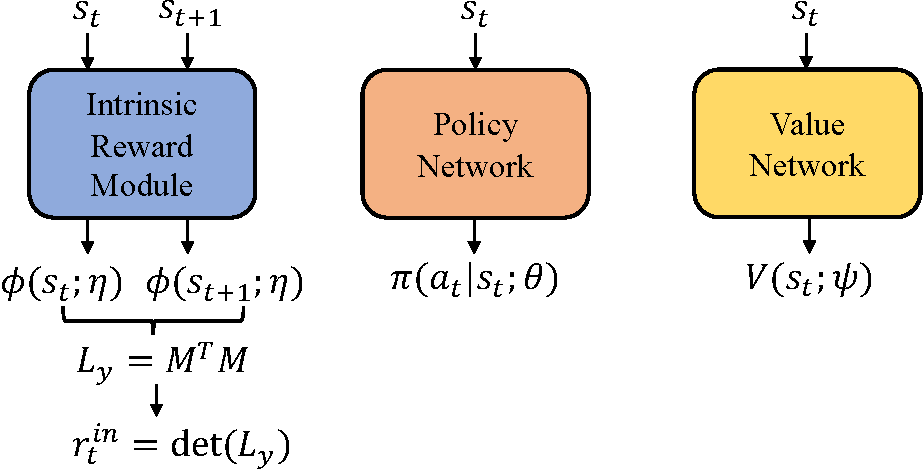
\includegraphics[width=0.7\linewidth]{figures/chapter5/daim-struct.pdf}
    \caption[Overview of three networks in DAIM.]{Overview of three networks in DAIM: intrinsic reward module, policy network, and value network.}
    \label{fig:structure_overview}
\end{figure}

\section{Experiments}
In this section, we evaluate $\ourmethod$ with different selections of baseline policy gradient architecture, namely, proximal policy optimisation (PPO) and advantage actor critic (A2C). We choose MuJoCo locomotion and the arcade learning environments (Atari games and SuperMarioBro) as the benchmark environments (see Figure~\ref{fig:ch5_envs}).
\begin{figure}[h]
    \begin{subfigure}{\textwidth}
        \centering
        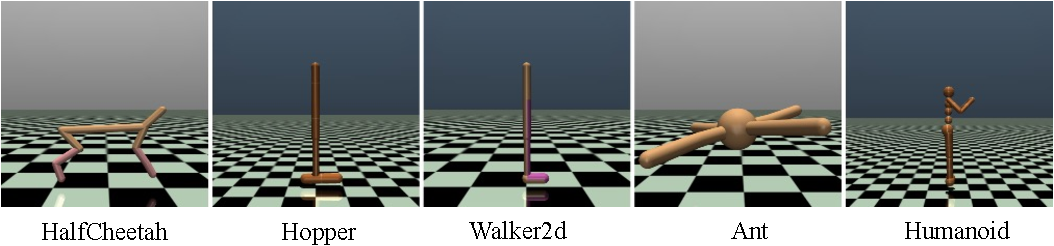
\includegraphics[width=0.9\textwidth]{figures/chapter5/mujoco_env.pdf}
        \caption{MuJoCo Locomotion Environment.}
        \label{fig:mujoco_env}
    \end{subfigure}
    \begin{subfigure}{\textwidth}
        \centering
        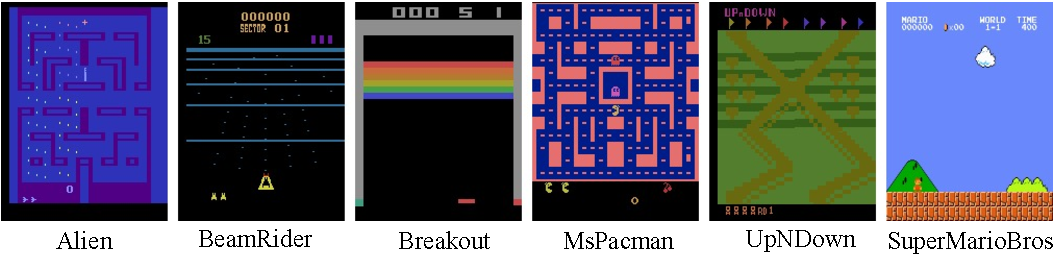
\includegraphics[width=0.9\textwidth]{figures/chapter5/atari_env.pdf}
        \caption{Arcade Learning Environment.}
        \label{fig:ale_env}
    \end{subfigure}
    \caption[Evaluation environments of DAIM.]{Visualisation of (a) MuJoCo Locomotion Environment: HalfCheetah, Hopper, Walker2d, Ant, and Humanoid, and (b) Arcade Learning Environment: Alien, BeamRider, Breakout, MsPacman, UpNDown, and SuperMarioBros.}
    \label{fig:ch5_envs}
\end{figure}

\subsection{Environments}
Firstly, we evaluate our agent in the MuJoCo locomotion environment~\cite{duan2016benchmarking} and use PPO as the base RL algorithm. We use two kinds of environment settings for evaluation: the standard setting and the delayed reward setting~\cite{zheng2018learning}. Specifically, {for the delayed reward setting}, the accumulated reward is only given every 10, 20 or 40 steps. This setting is more difficult for agent learning. The five tasks selected in the experiment are HalfCheetah, Hopper, Walker2d, Ant and Humanoid (see Figure~\ref{fig:mujoco_env}).

Subsequently, to investigate the performance of $\ourmethod$ with high dimensional inputs, we also evaluate our approach on the Atari games and the SuperMarioBros~\cite{gym-super-mario-bros} using A2C as our base RL algorithm. For the Atari games, Alien, BeamRider, Breakout, MsPacman and UpNDown are selected as our test bench (see Figure~\ref{fig:ale_env}). 

\subsection{Experimental Settings}
In MuJoCo tasks, baseline methods are vanilla PPO~\cite{schulman2017proximal}, LIRPG~\cite{zheng2018learning} and VIME~\cite{NIPS2016_abd81528}. The intrinsic module $\phi_{\eta}(\cdot)$ has 3 hidden layers with 64 neurons with ReLU activation functions. The output of the intrinsic module is a 64 dimensional embedding feature. Adam~\cite{kingma2014adam} is chosen as the optimiser with learning rate $\alpha=0.0001$. $\lambda^{\text{in}}$ and $\lambda^{\text{ex}}$ are both set to 1 as default. The hyperparameters of PPO part are kept the same as the baseline setting: timesteps per rollout are 2048, clip ratio is 0.2, entropy coefficient is 0, optimisation epochs per iteration is 10, batch size is 64, learning rate is 0.0003, discount factor $\gamma$ is 0.99, and GAE parameter $\lambda$ is 0.95. Training for each agent lasts for 1 million frames. {The average time of one complete training run of DAIM using one random seed on the MuJoCo tasks is 1.46 hours.}

In the Atari games and SuperMarioBros, Vanilla A2C and LIRPG are selected as baseline methods. For $\ourmethod$, the same CNN architecture as A2C is used within the intrinsic module, with a 256-dimensional feature vector as output. RMSprop is selected as the optimiser with learning rate $\alpha=0.0007$. $\lambda^{\text{in}}$ and $\lambda^{\text{ex}}$ are set to 0.01 and 1 respectively. The hyperparameters of the A2C part are kept the same as the baseline setting: number of workers is 16, timesteps per rollout of each worker are 5, entropy coefficient is 0.01, learning rate is 0.0007, discount factor $\gamma$ is 0.99, and GAE parameter $\lambda$ is 0.95. Training on the Atari games and SuperMarioBros lasts for 50 million and 5 million frames respectively. One complete training run of DAIM using one random seed takes 23.96 hours and 2.83 hours on the Atari games and the SuperMarioBros, respectively.

\subsection{Results on MuJoCo Locomotion Environment}
The comparisons between DAIM and baselines are presented in Figure~\ref{fig:mujoco_results} and the related quantitative results are in Table~\ref{tab:standard} and Table~\ref{tab:delay}. In the standard setting, $\ourmethod$ achieves higher rewards than PPO and VIME in 4 out of 5 tasks, and outperforms LIRPG on all tasks. We notice that in the standard setting without delay, LIRPG has similar or lower performance than PPO. This might be because in the standard setting -- which uses dense rewards -- the agent can receive an extrinsic reward at each timestep and LIRPG does not encourage any exploration explicitly. Thus, the learned intrinsic rewards {of LIRPG} provide only minor contributions. 

In the delayed reward setting, $\ourmethod$ achieves the best performance in 12 cases out of 15 delayed reward tasks. This indicates that, through the bi-level update, $\ourmethod$ still maximises the accumulated rewards, so the performance does not drop. On the other hand, it also suggests that the diversity-based intrinsic rewards help training in delayed-reward environments. Due to only receiving delayed rewards, the performance of PPO drops with the increase of the delay period. LIRPG and VIME can achieve better results than PPO, because they can provide the intrinsic reward to the agent at each step. The result shows that $\ourmethod$ adopts DPPs as a diversity measure between states, which encourages the agent to explore in the environment even with only delayed rewards.

In addition, we also investigate the performance of $\ourmethod$ under different reward weights, $\lambda^{\text{ex}}=\{0.01, 0\}$. When $\lambda^{\text{ex}}=0$, the policy is updated towards maximising the intrinsic reward only. From Figure~\ref{fig:mujoco_results}, either $\lambda^{\text{ex}}=0$ or $\lambda^{\text{ex}}=0.01$, the results achieved are comparable to $\lambda^{\text{ex}}=1$ in both the standard and delayed reward settings. More specifically, the weight coefficients $\lambda^{\text{ex}}$ and $\lambda^{\text{in}}$ determine which reward plays the major role during training.  When $\lambda^{\text{ex}}=1$, the agent can outperform other baselines in most tasks, especially in the standard and the delayed reward setting with a short delay (Delay = 10). In these settings, the extrinsic rewards can provide feedback frequently which is helpful to the training. But in the tasks with longer delayed feedback ({e.g.}, Delay=20 and Delay=40), the extrinsic rewards only rarely provide useful feedback, and the intrinsic rewards -- which can provide denser feedback -- lend valuable guidance to the agent. Thus, reducing the weighting of the extrinsic rewards can sometimes improve the performance of the agent, though this depends on the dynamics of the particular environment (see Figure~\ref{fig:mujoco_results}).

This also demonstrates that the bi-level update has led to meaningful intrinsic {rewards} that can criticize the policy.
\begin{figure}[t!]
    \centering
    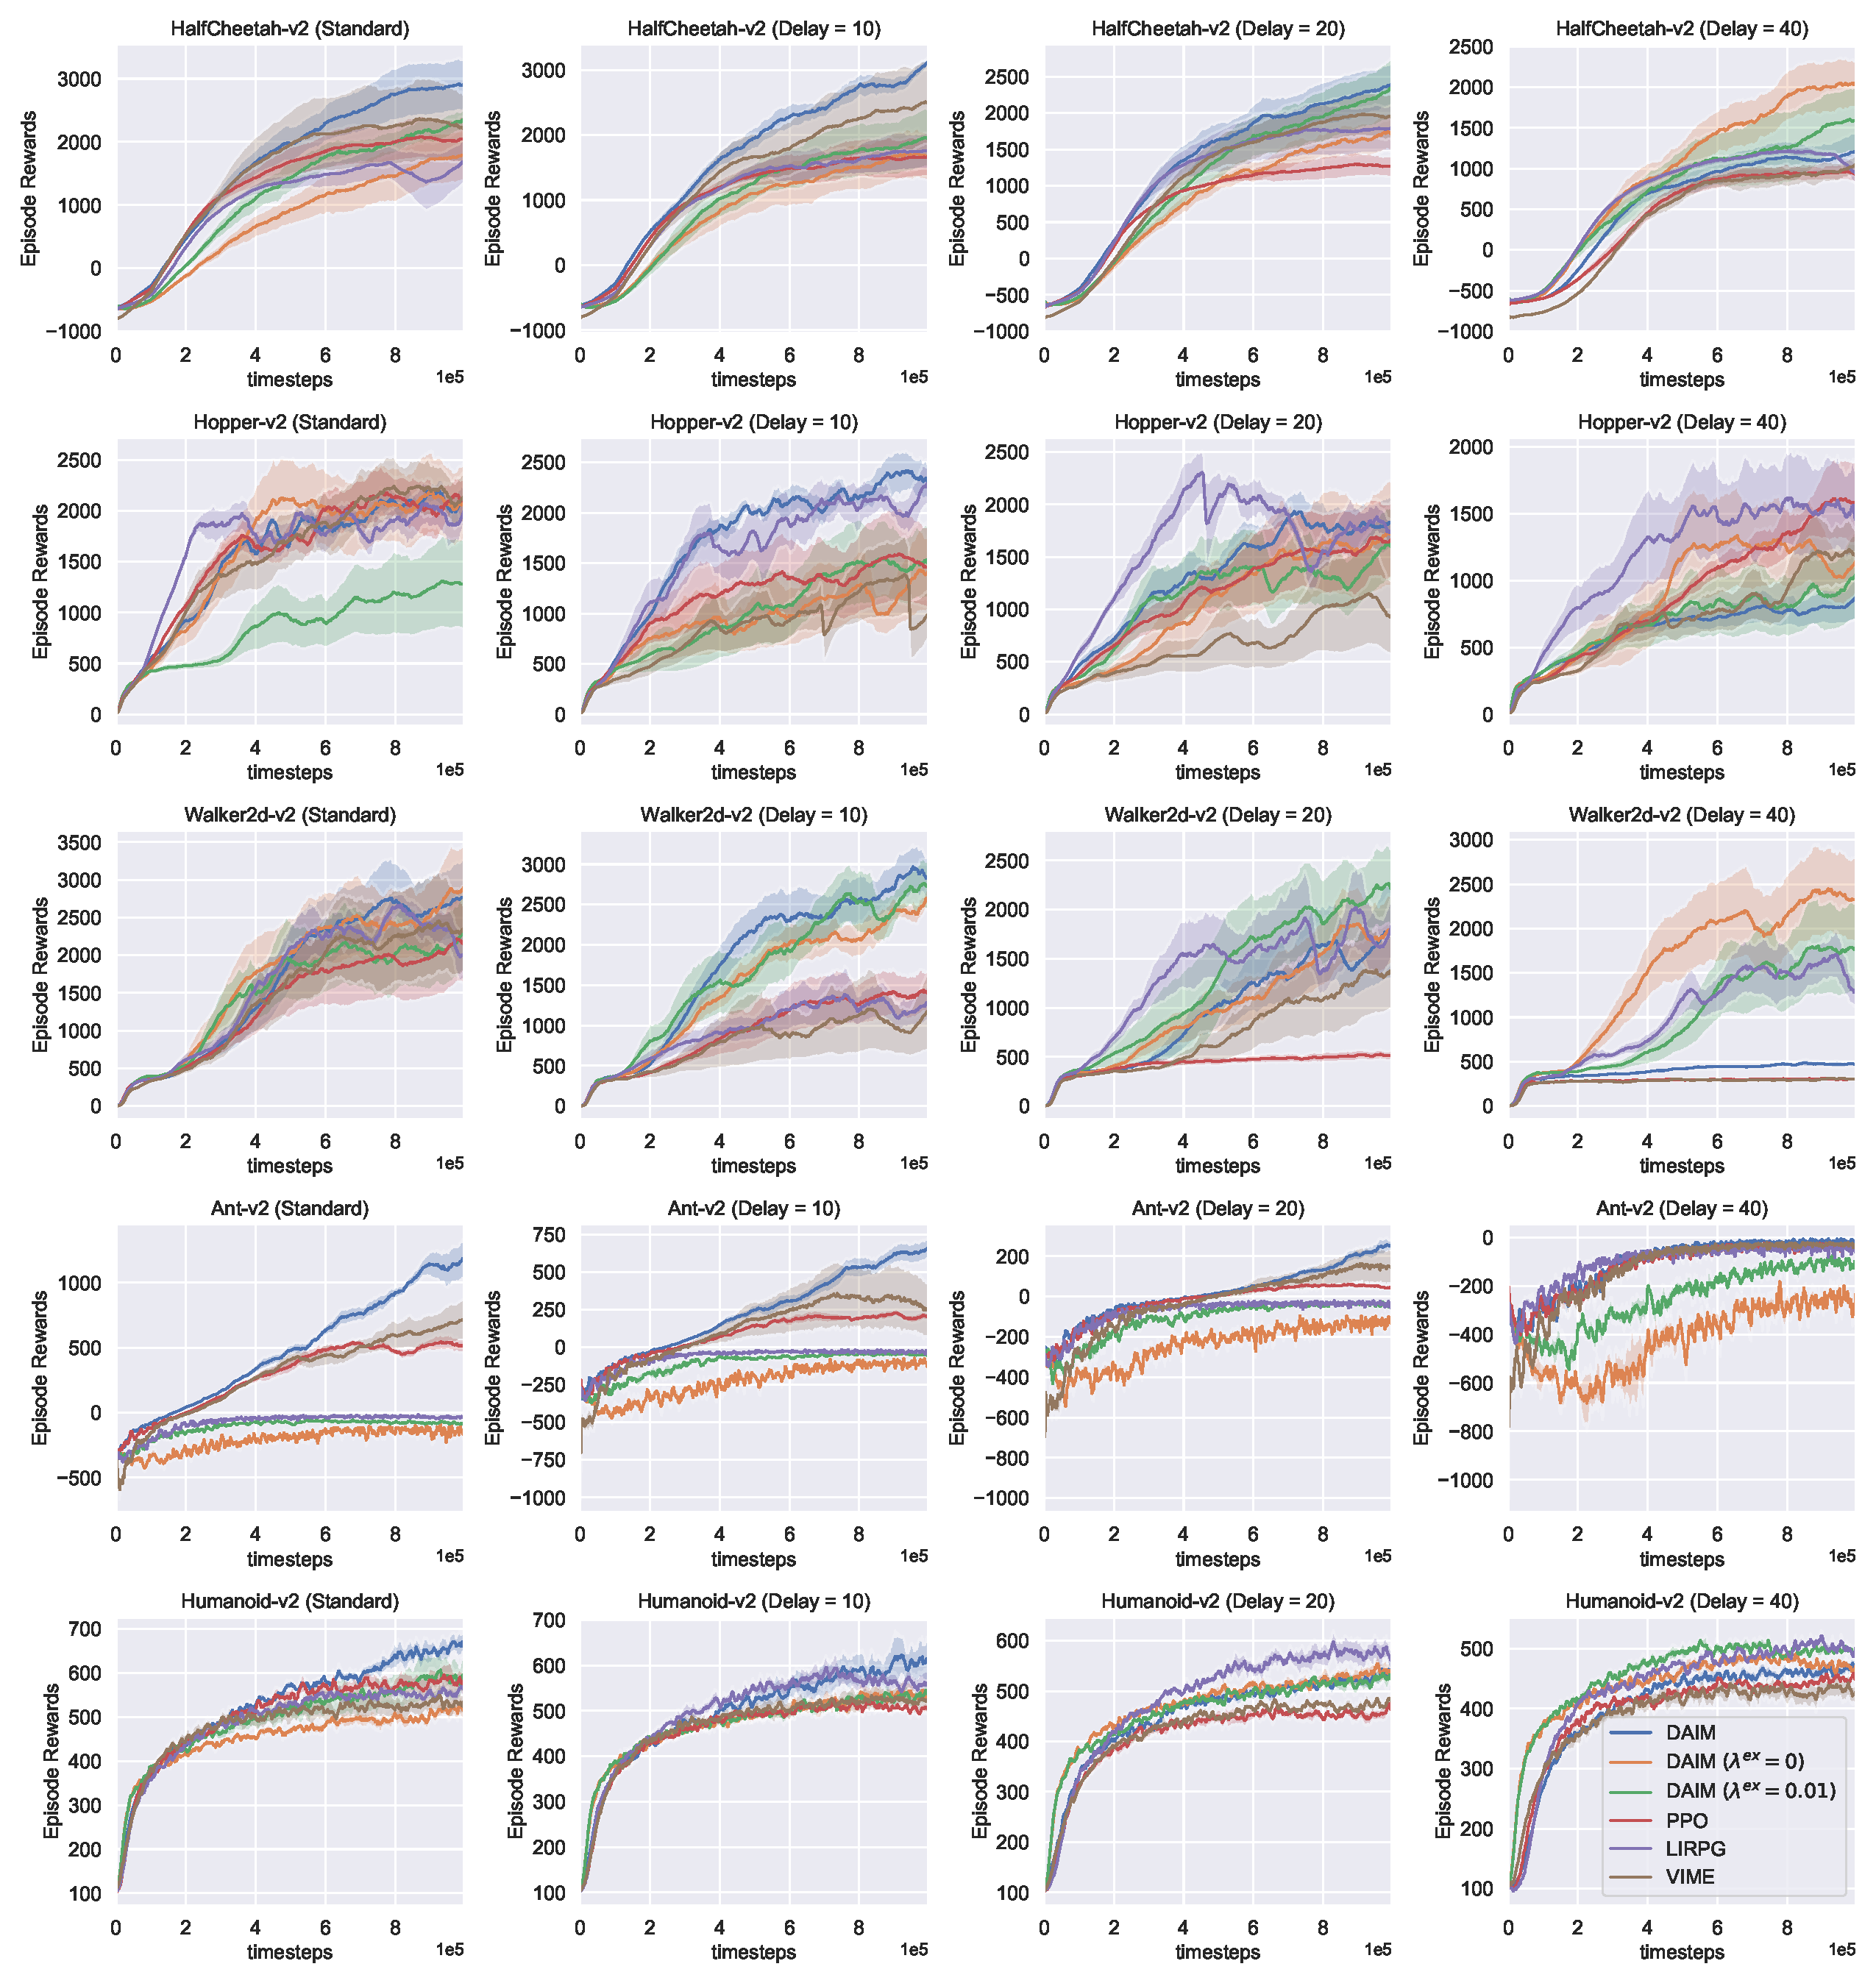
\includegraphics[width=1.0\linewidth]{figures/chapter5/mujoco_result_54_seaborn.pdf}
    \caption[Results of DAIM in the MuJoCo environment with standard and delayed reward settings.]{Comparison between $\ourmethod$ and baseline approaches (PPO, LIRPG, and VIME) in the MuJoCo locomotion environment with standard and delayed reward settings. The $x$-axis represents the number of timesteps in training. The $y$-axis represents the average extrinsic rewards over the last 100 training episodes. All of the experiments were run using 5 different seeds. The solid lines and shaded areas in the plots represent the mean and the standard errors over the performances of the different seeds.}
    \label{fig:mujoco_results}
\end{figure}

\begin{table}[h!]
    \centering
    \resizebox{0.9\textwidth}{!}{
    \begin{tabular}{c|ccccc}
    \toprule
     \multirow{2}{*}{Methods} & \multicolumn{5}{c}{Standard} \\
     \cmidrule(lr){2-6}
         & HalfCheetah & Hopper & Walker2d & Ant & Humanoid \\
    \midrule
    PPO & 2039$\pm$354 & \underline{2112$\pm$208} & 2145$\pm$514 & {512$\pm$53} & 566$\pm$28\\
    LIRPG & 1694$\pm$347 & 2004$\pm$125 & 1997$\pm$322 & -25$\pm$3 & 562$\pm$14 \\
    VIME & 2204$\pm$545 & \textbf{2126$\pm$238} & 2323$\pm$562 & \underline{711$\pm$157} & 530$\pm$29 \\
    \midrule
    DAIM & \textbf{2895$\pm$405} & {2103$\pm$129} & \underline{2766$\pm$487} & \textbf{1192$\pm$157} & \textbf{670$\pm$23} \\
    DAIM ($\lambda^{ex}=0$) & 1780$\pm$405 & 2078$\pm$377 & \textbf{2879$\pm$580} & -164$\pm$35& 516$\pm$19\\
    DAIM ($\lambda^{ex}=0.01$) & \underline{2363$\pm$158} & 1290$\pm$442 & 2285$\pm$504 & -84$\pm$12 & \underline{593$\pm$39}\\
    \bottomrule
    \end{tabular}
    }
    \caption[Average reward of DAIM in the MuJoCo environments with the standard reward setting in the final epoch during training.]{Quantitative results comparison between DAIM and other baseline methods (PPO, LIRPG, and VIME) in the MuJoCo locomotion environment with the standard reward setting. In the table, it shows final average extrinsic rewards $\pm$ standard error across 5 different seeds of last 100 episodes in the training. The best and the second best results are (\textbf{bold}) and (\underline{underline}), respectively.}
    \label{tab:standard}
\end{table}

\begin{table}[h!]
    \centering
    \resizebox{0.9\textwidth}{!}{
    \begin{tabular}{c|ccccc}
    \toprule
     \multirow{2}{*}{Methods} & \multicolumn{5}{c}{ Delay = 10} \\
     \cmidrule(lr){2-6}
      & HalfCheetah & Hopper & Walker2d & Ant & Humanoid \\
    \midrule
    PPO & 1674$\pm$297& 1457$\pm$396 & 1404$\pm$258 & {207$\pm$26} & 503$\pm$9 \\
    LIRPG & 1756$\pm$273 & \underline{2275$\pm$192} & 1279$\pm$215 &-27$\pm$5 & \underline{555$\pm$31} \\
    VIME & \underline{2498$\pm$638} & 992$\pm$232 & 1186$\pm$487 & \underline{249$\pm$182} & 518$\pm$24 \\
    \midrule
    DAIM & \textbf{3114$\pm$72} & \textbf{2288$\pm$181} & \textbf{2824$\pm$248} & \textbf{663$\pm$67} & \textbf{612$\pm$45} \\
    DAIM ($\lambda^{ex}=0$) &1680$\pm$367&1420$\pm$371 &2582$\pm$116 &-97$\pm$30 & 530$\pm$20 \\
    DAIM ($\lambda^{ex}=0.01$) & {1961$\pm$450} & 1495$\pm$368& \underline{2730$\pm$307}& -51$\pm$15 & 535$\pm$24\\
    \midrule
    \midrule
    \multirow{2}{*}{Methods} & \multicolumn{5}{c}{ Delay = 20} \\
     \cmidrule(lr){2-6}
      & HalfCheetah & Hopper & Walker2d & Ant & Humanoid \\
    \midrule
    PPO & 1274$\pm$148 & 1672$\pm$358 & 519$\pm$49 & {45$\pm$11} & 458$\pm$16 \\
    LIRPG & 1790$\pm$317& \underline{1748$\pm$127} & \underline{1835$\pm$313} &-50$\pm$8 & \textbf{568$\pm$20} \\
    VIME & 1948$\pm$308 & 936$\pm$354 & 1368$\pm$379 & \underline{142$\pm$86} & 477$\pm$5 \\
    \midrule
    DAIM & \textbf{2397$\pm$288} & \textbf{1810$\pm$236} & 1792$\pm$483 & \textbf{249$\pm$25}& \underline{545$\pm$24} \\
    DAIM ($\lambda^{ex}=0$) & 1736$\pm$244 & 1734$\pm$505 &1809$\pm$357 & -172$\pm$32 & 539$\pm$17 \\
    DAIM ($\lambda^{ex}=0.01$) & \underline{2350$\pm$413} & 1586$\pm$353 & \textbf{2209$\pm$406} & -40$\pm$4 & 527$\pm$14 \\
    \midrule
    \midrule
    \multirow{2}{*}{Methods} & \multicolumn{5}{c}{ Delay = 40} \\
     \cmidrule(lr){2-6}
      & HalfCheetah & Hopper & Walker2d & Ant & Humanoid \\
    \midrule
    PPO & 931$\pm$113 & \textbf{1590$\pm$300} & 305 $\pm$13 & {-50$\pm$9} & 449$\pm$7 \\
    LIRPG & 941$\pm$130 & \underline{1456$\pm$359}& 1292$\pm$169 & -51$\pm$13 & \textbf{502$\pm$6}\\
    VIME  & 1053$\pm$121 & 1178$\pm$173 & 304$\pm$14 & \underline{-26$\pm$11} & 425$\pm$16 \\
    \midrule
    DAIM & 1201$\pm$126& 879$\pm$166 & 476$\pm$38 & \textbf{-13$\pm$6} & 467$\pm$13\\
    DAIM ($\lambda^{ex}=0$) & \textbf{2034$\pm$283} & 1153$\pm$248 & \textbf{2324$\pm$475} & -208$\pm$24 & 473$\pm$6\\
    DAIM ($\lambda^{ex}=0.01$) & \underline{1597$\pm$410} & 1052$\pm$337 & \underline{1768$\pm$518}& -117$\pm$19 & \underline{488$\pm$7}\\
    \bottomrule
    \end{tabular}}
    \caption[Average reward of DAIM in the MuJoCo environments with the delayed reward settings in the final epoch during training.]{Quantitative results comparison between DAIM and other baseline methods (PPO, LIRPG, and VIME) in the MuJoCo locomotion environment with the delayed reward setting. In the table, it shows final average extrinsic rewards $\pm$ standard error across 5 different seeds of last 100 episodes in the training. The best and the second best results are (\textbf{bold}) and (\underline{underline}), respectively.}
    \label{tab:delay}
\end{table}

% \begin{figure}[t!]
% % \vspace{-1.cm}
%     \centering
%     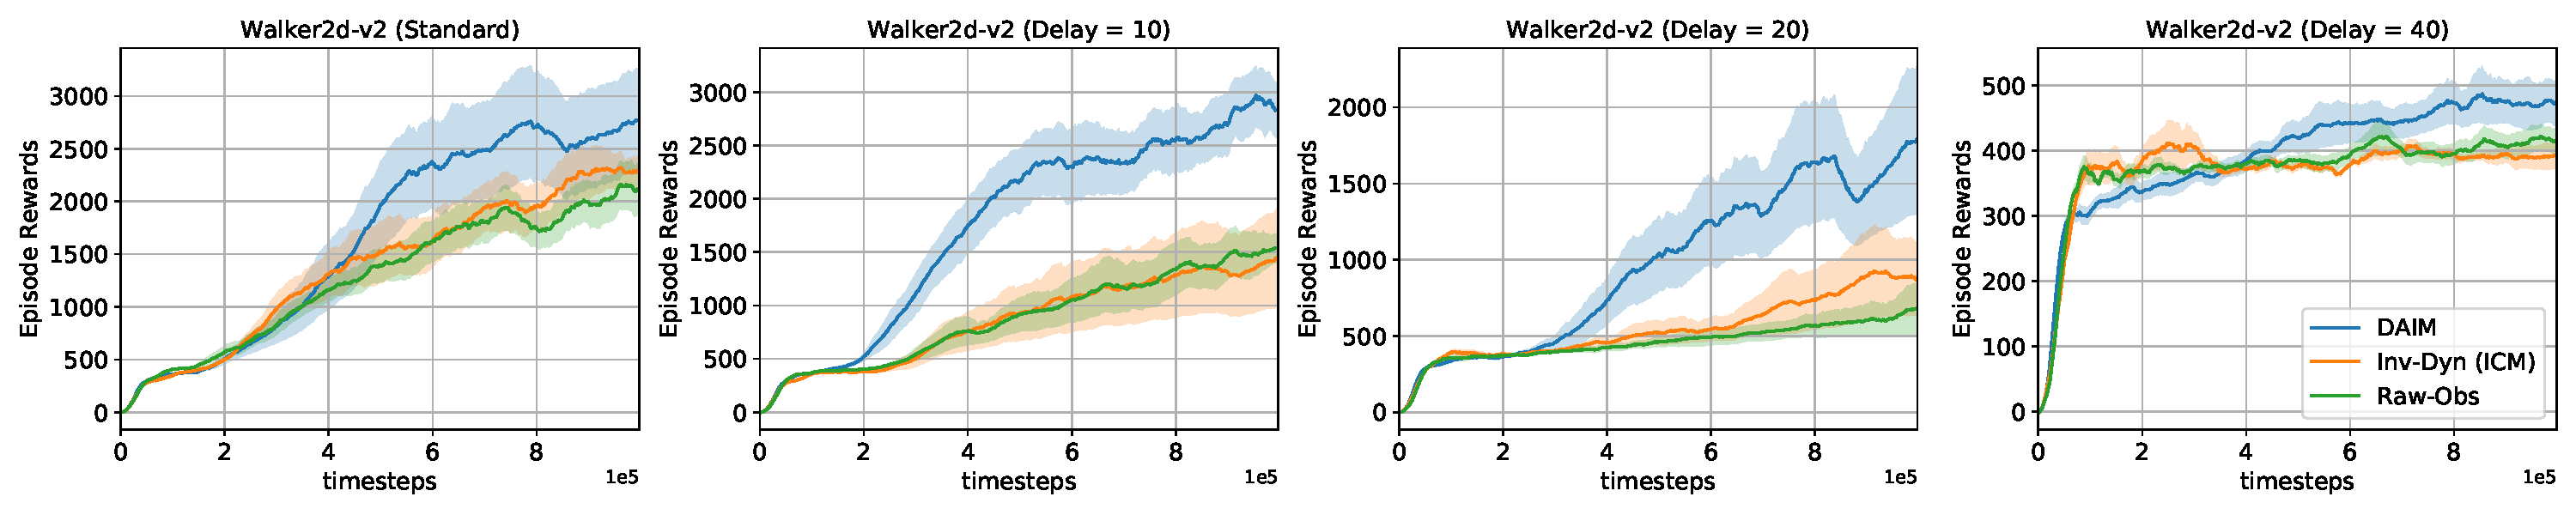
\includegraphics[width=\linewidth]{figures/chapter5/walker2d_result.pdf}
%     \caption{The performance of different feature embedding methods in the Walker2d task with standard and delayed reward settings. DAIM achieves higher accumulated extrinsic rewards.}
%     \label{fig:walker2d_results}
% \end{figure}
\begin{figure}[h!]
\centering
  \begin{subfigure}[t]{0.49\textwidth}
    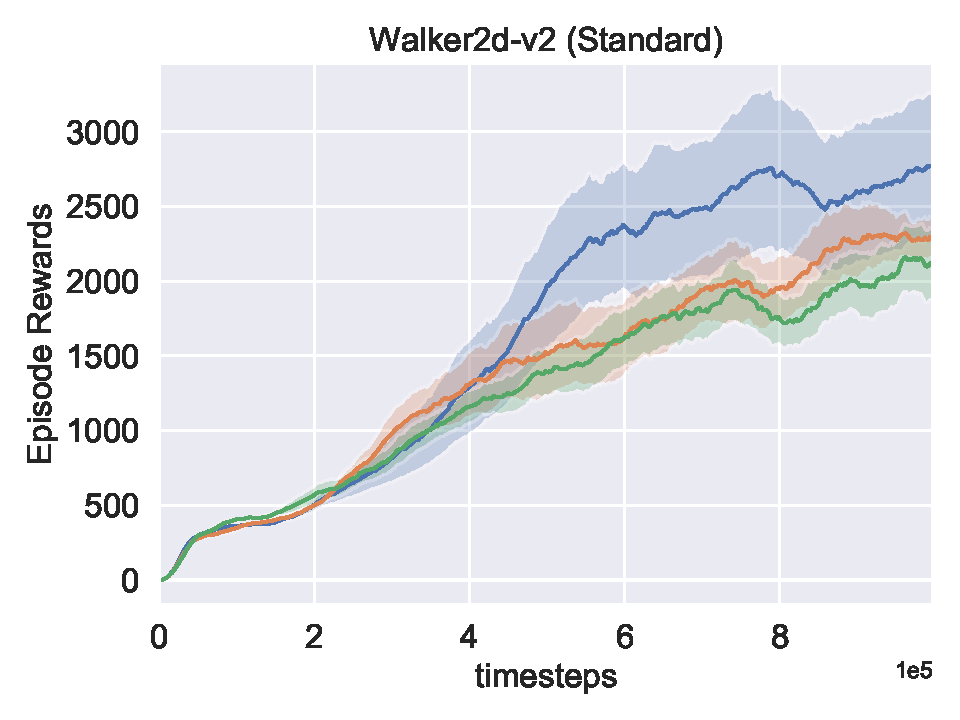
\includegraphics[width=\textwidth]{figures/chapter5/embedding/delay1.pdf}
    \caption{Standard}
  \end{subfigure}\hfill
  \begin{subfigure}[t]{0.49\textwidth}
    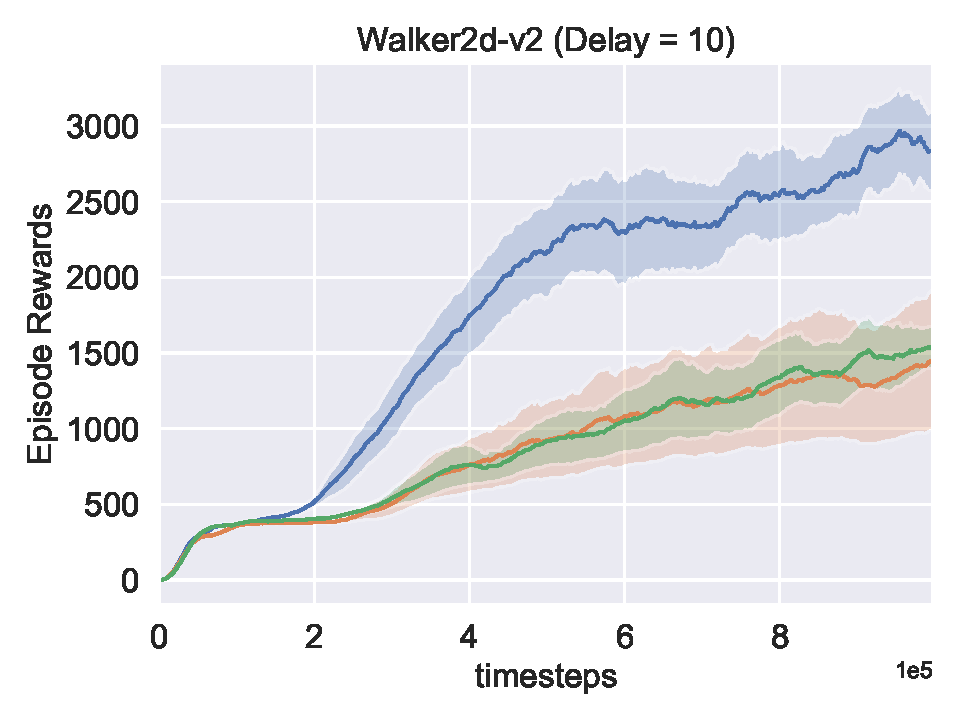
\includegraphics[width=\textwidth]{figures/chapter5/embedding/delay10.pdf}
    \caption{Delay=10}
  \end{subfigure}\hfill
  \begin{subfigure}[t]{0.49\textwidth}
    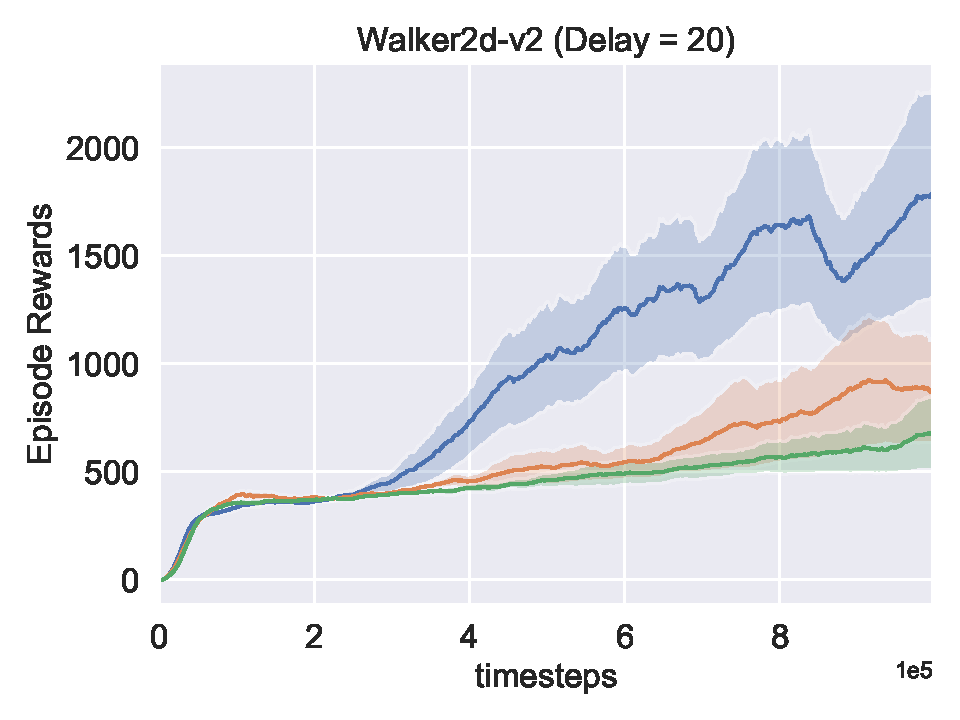
\includegraphics[width=\textwidth]{figures/chapter5/embedding/delay20.pdf}
    \caption{Delay=20}
  \end{subfigure}\hfill
  \begin{subfigure}[t]{0.49\textwidth}
    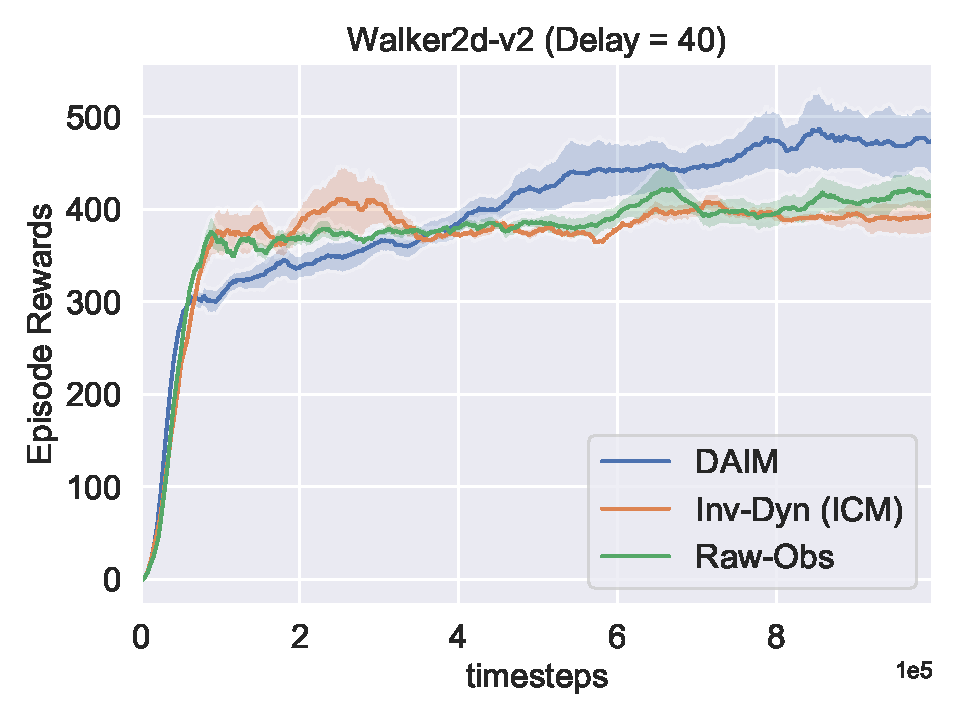
\includegraphics[width=\textwidth]{figures/chapter5/embedding/delay40.pdf}
    \caption{Delay=40}
  \end{subfigure}\hfill
  \caption[Results of different feature embedding methods in the Walker2d task with standard and delayed reward settings.]{The performance of different feature embedding methods in the Walker2d task with standard and delayed reward settings. DAIM achieves higher accumulated extrinsic rewards.} 
  \label{fig:walker2d_results}
\end{figure}
% \begin{figure}[t!]
%     \centering
%     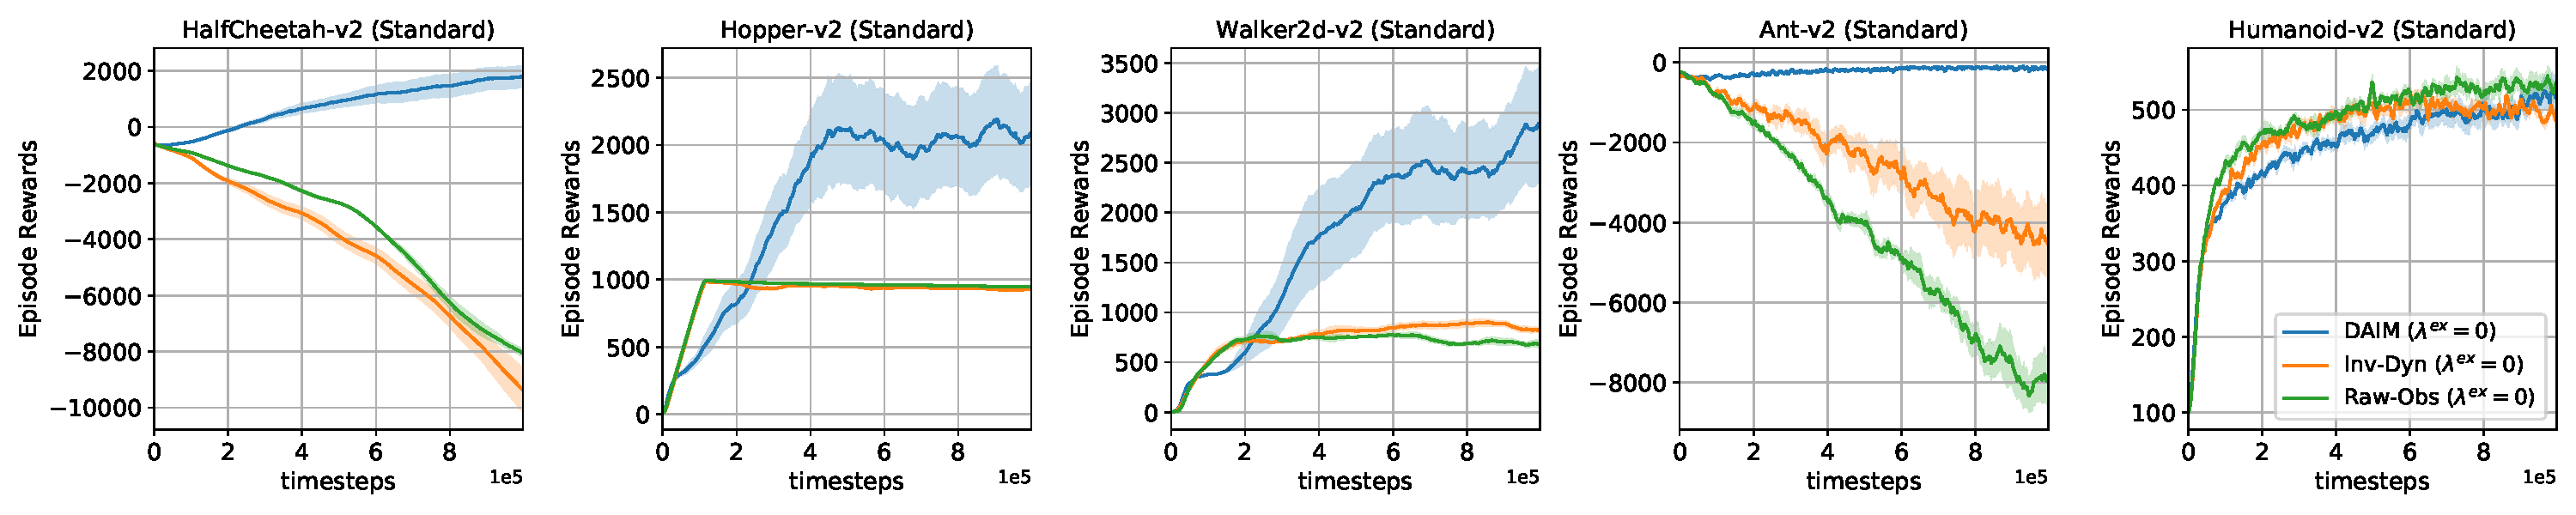
\includegraphics[width=\linewidth]{figures/chapter5/walker2d_r_in_result.pdf}
%     \caption{Using {\em only} intrinsic rewards ($\lambda^{\text{ex}}=0$), we evaluate the performance (accumulated {\it extrinsic} rewards on vertical axes) of different feature embedding methods in all five MuJoCo tasks with the standard reward setting.}
%     \label{fig:walker2d_results_r_in}
% \end{figure}
\begin{figure}[h!]
\centering
  \begin{subfigure}[t]{0.49\textwidth}
    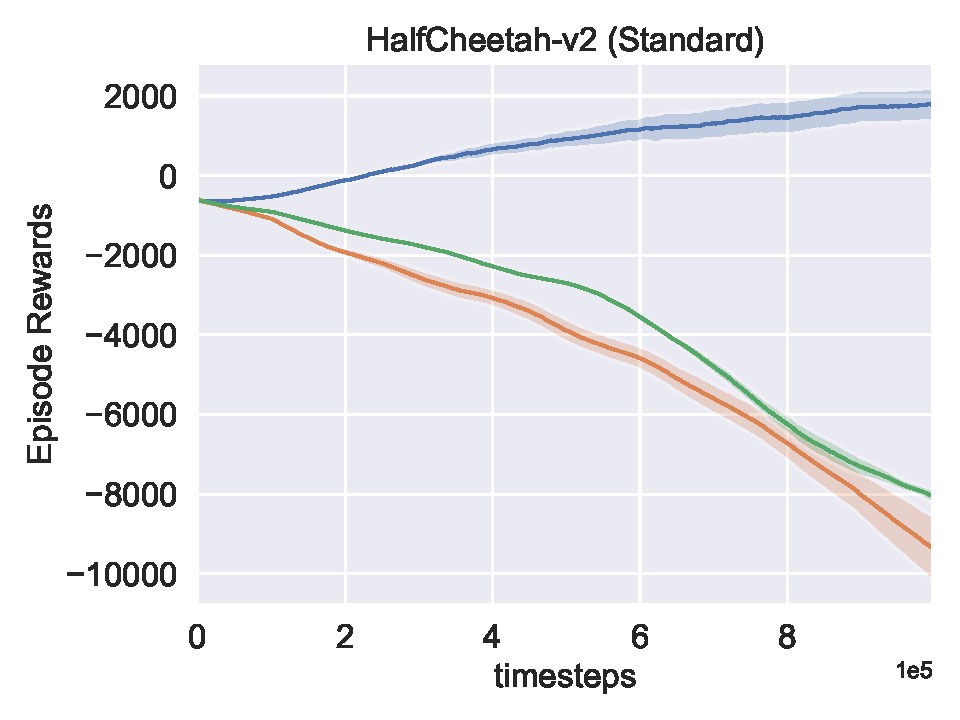
\includegraphics[width=\textwidth]{figures/chapter5/r_in_only/halfcheetah.pdf}
    \caption{HalfCheetah}
  \end{subfigure}\hfill
  \begin{subfigure}[t]{0.49\textwidth}
    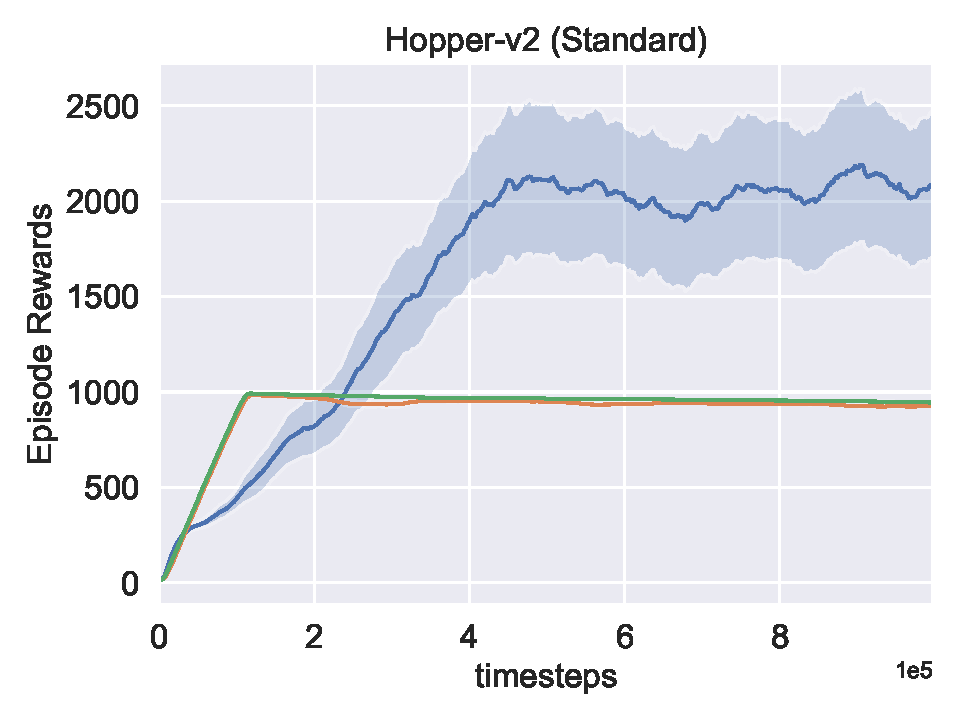
\includegraphics[width=\textwidth]{figures/chapter5/r_in_only/hopper.pdf}
    \caption{Hopper}
  \end{subfigure}\hfill
  \begin{subfigure}[t]{0.49\textwidth}
    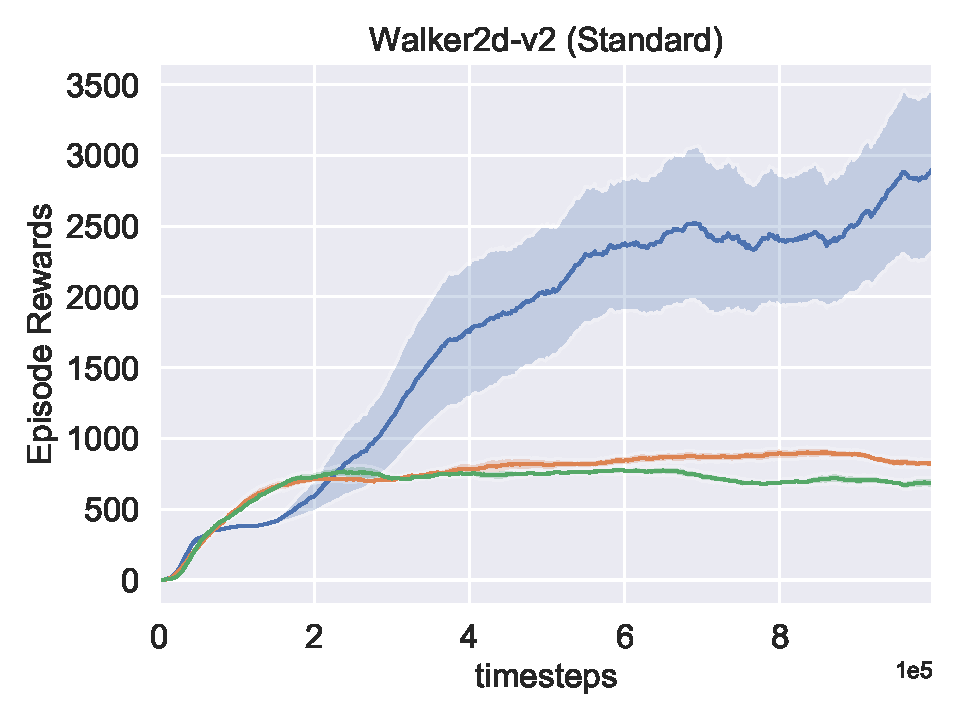
\includegraphics[width=\textwidth]{figures/chapter5/r_in_only/walker2d.pdf}
    \caption{Walker2d}
  \end{subfigure}\hfill
  \begin{subfigure}[t]{0.49\textwidth}
    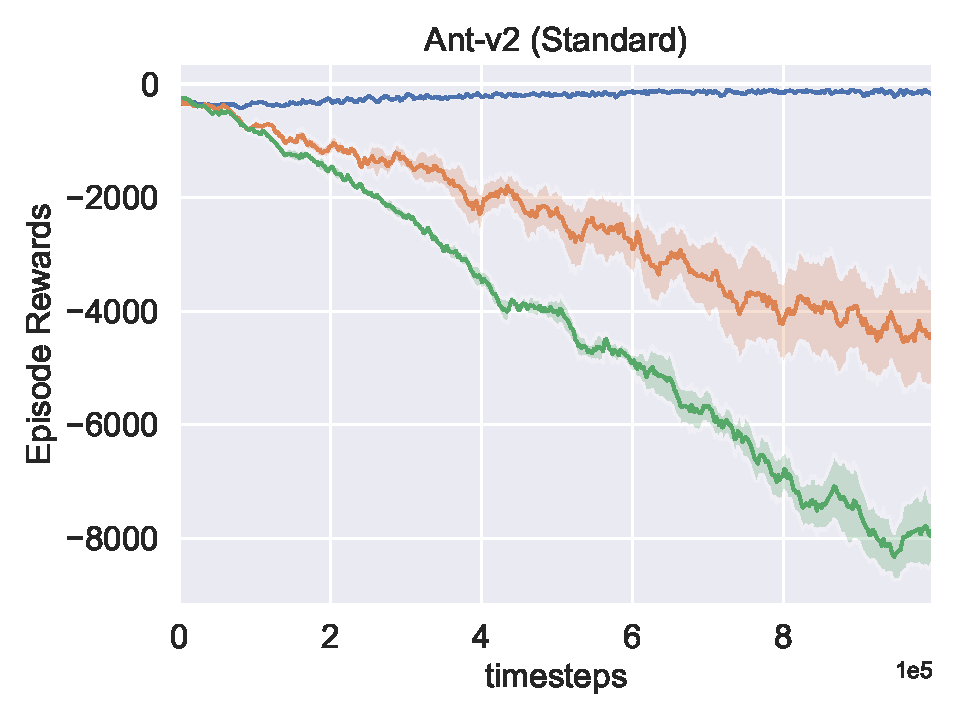
\includegraphics[width=\textwidth]{figures/chapter5/r_in_only/ant.pdf}
    \caption{Ant}
  \end{subfigure}\hfill
  \begin{subfigure}[t]{0.49\textwidth}
    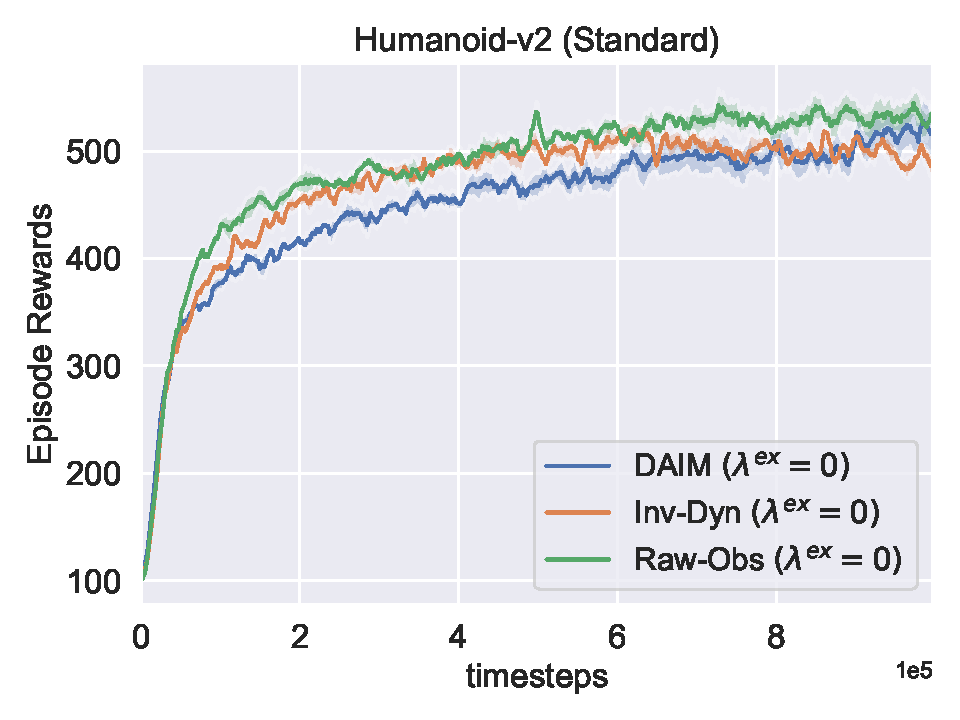
\includegraphics[width=\textwidth]{figures/chapter5/r_in_only/humanoid.pdf}
    \caption{Humanoid}
  \end{subfigure}\hfill
  \caption[Results of using intrinsic reward only with different feature embedding methods in the MuJoCo environment with the standard reward setting.]{Using {\em only} intrinsic rewards ($\lambda^{\text{ex}}=0$), we evaluate the performance (accumulated {\it extrinsic} rewards on vertical axes) of different feature embedding methods in all five MuJoCo tasks with the standard reward setting.} 
  \label{fig:walker2d_results_r_in}
\end{figure}


\subsubsection{Feature Embedding Methods Study}
We also investigate the efficiency of the other two feature learning methods as our baselines which are summarized briefly as below.

\noindent\textbf{Inverse Dynamics Features} (\text{Inv-Dyn}) Pathak \textit{et al.}~\cite{pathak2017curiosity} propose the inverse dynamics model in the Intrinsic Curiosity Module (ICM). The inverse dynamics model uses the current state $s_{t}$ and the next state $s_{t+1}$ to predict the action $a_{t}$. The motivation of this method is that the learned features should only depends on the current action of the agent: theoretically, it would not be affected by insignificant changes in the environment. The predicted action $a_{t}$ is estimated by:
\begin{equation}
    \widehat{a_{t}} = g(\phi(s_{t};\eta), \phi(s_{t+1};\eta);\theta_{I}),
\end{equation}
where, $g$ is the inverse dynamics model and $\phi(\cdot;\eta)$ is the learned embedding feature space. The parameters of the embedding network, $\eta$, and the parameters of the inverse dynamic model $\theta_{I}$ are optimised through minimising the error of the predicted action $\widehat{a_{t}}$ and the actual action $a_{t}$:
\begin{equation}
    \min_{\eta, \theta_{I}}\mathcal{L}(\widehat{a_{t}}, a_{t}),
\end{equation}
In the MuJoCo tasks, the action space is continuous and the output of the inverse dynamics model $g$ is the mean $\mu$ and standard deviation $\sigma$ of the Gaussian distribution over the action space. The loss function $\mathcal{L}$ is used to minimise the discrepancy between the predicted action $\widehat{a_{t}}$ and the actual action $a_{t}$ through maximising the log-likelihood estimation of $\theta_{I}$ under the Gaussian distribution.

\noindent\textbf{Raw Observation Features} (\text{Raw-Obs}) We also adopt a simple way to calculate the intrinsic reward as a baseline. The raw observations are used directly, where $\phi(s_{t})=s_{t}$. However, this method is subject to observation noises and cannot scale to high-dimensional inputs.

In Figure~\ref{fig:walker2d_results}, we compare the performance of all feature embedding methods in the Walker2d task with and without delayed rewards. $\ourmethod$ achieves the best results in the standard and delayed reward settings, whereas the other two feature embedding methods have similar performance. It must be emphasised that during the training of the feature embedding module of $\ourmethod$, the {\em intrinsic} network is updated to maximise the {\em extrinsic} returns. In this way, the learned features are likely to help the agent explore in an appropriate direction, which not only increases the diversity between the states but also leads to higher extrinsic returns. For \text{Inv-Dyn} and \text{Raw-Obs}, the dissimilarity between the adjacent states is only used as an intrinsic reward but not attempting to maximise extrinsic returns. In this case, the agent will maximise the diversity regardless of its effect on overall performance in terms of the extrinsic returns. For example, in Figure~\ref{fig:why_daim}, the agent selects an action in $s_{t}$, which causes it to fall into a trap in $s_{t+1}$. When the raw observation feature is used as the feature embedding method, the selected action leads to high diversity between the adjacent states, however the agent fails in this episode. Therefore, simply increasing diversity may not lead to better performance and it is necessary to learn the features that can better quantify the diversity between adjacent states to improve the task-specific performance (i.e., extrinsic returns) of the agent.

\begin{figure}[h]
    \centering
    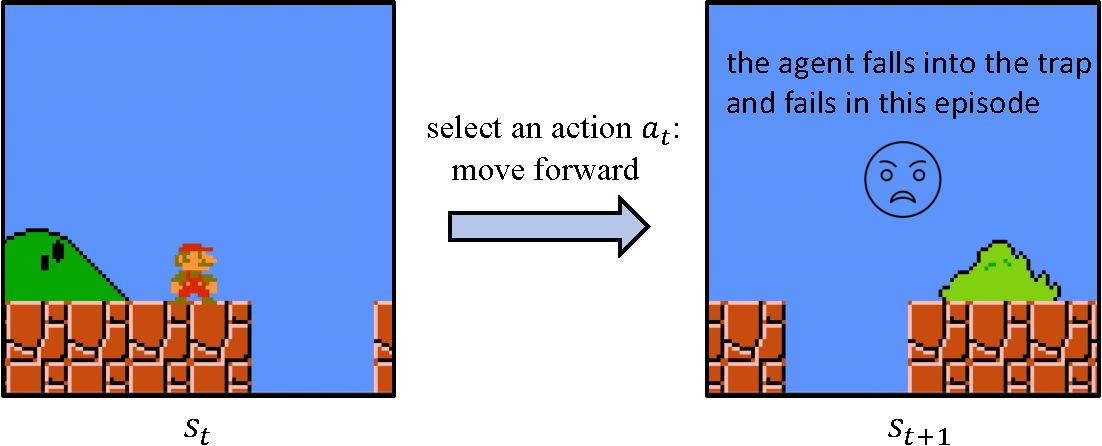
\includegraphics[width=0.9\textwidth]{figures/chapter5/diversity_fail.pdf}
    \caption{An example to show that higher diversity may not lead to better performance.}
    \label{fig:why_daim}
\end{figure}

We also train the agents with only intrinsic rewards, and results are shown in Figure~\ref{fig:walker2d_results_r_in}. $\ourmethod$ outperforms \text{Inv-Dyn} and \text{Raw-Obs}, which shows that higher diversity does not necessarily lead to better performance. In the standard reward setting, $\ourmethod$ yields higher rewards than the other two embedding feature methods in 4 out of 5 tasks. In the Ant task, the agent trained with inverse dynamic features and raw observation features yields decreasing performance. This suggests that the intrinsic reward is not, on its own, sufficient to train the agent. However, the features learned by using bi-level optimisation help to maximise the extrinsic returns, showing better performance than the other two methods.

% \begin{figure}[t!]
%     \centering
%     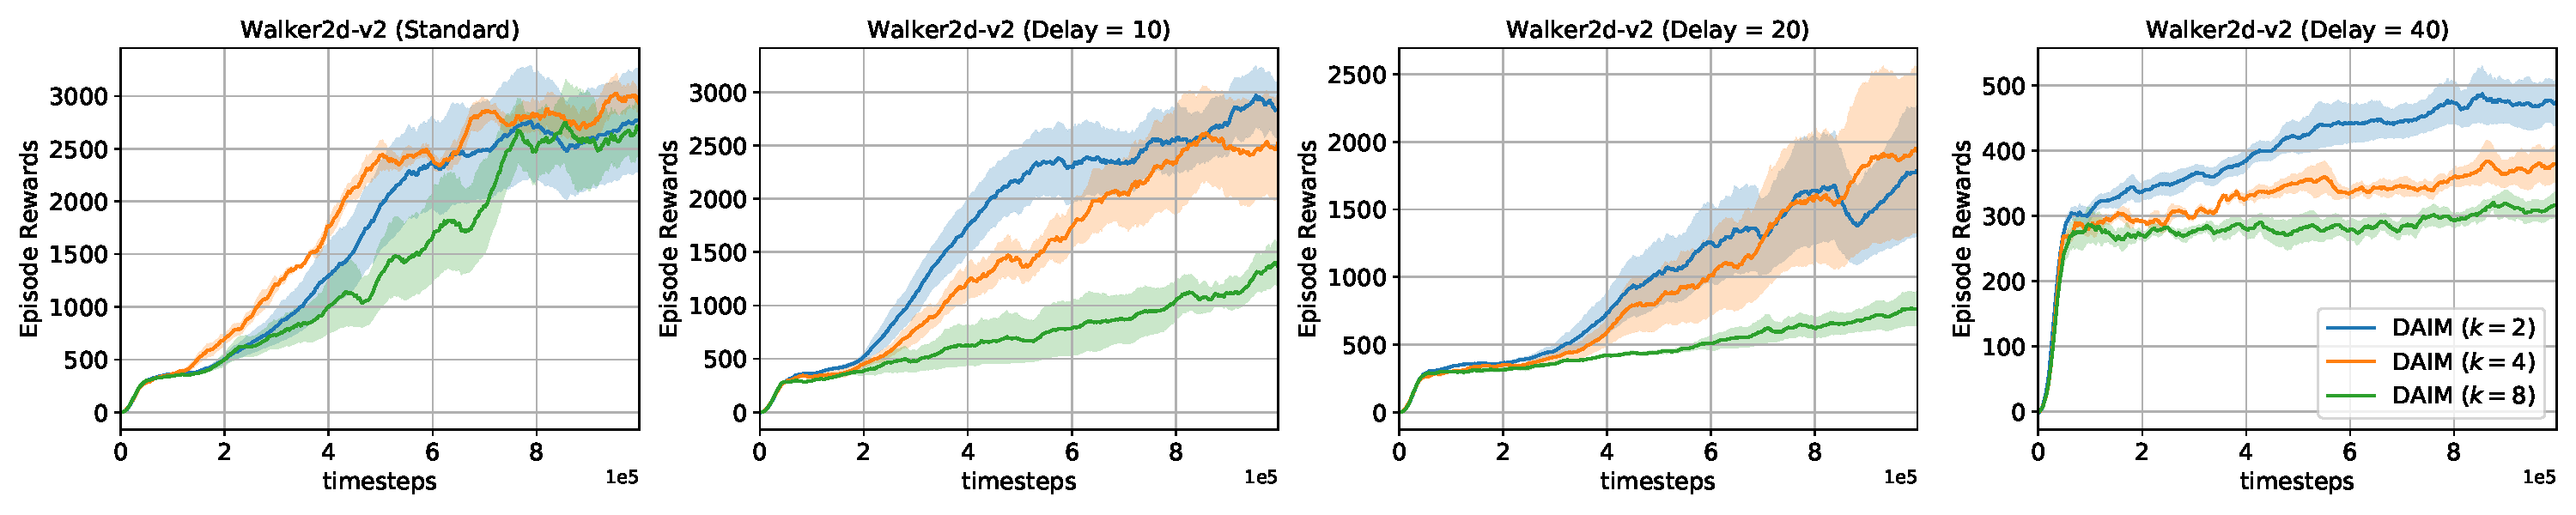
\includegraphics[width=\linewidth]{figures/chapter5/mujoco_kernel_ablation.pdf}
%     \caption{The performance of using different size $k$ of consecutive states for calculating intrinsic rewards in the Walker2d task with standard and delayed reward settings.  The $y$-axis represents the average extrinsic rewards over the last 100 training episodes.}
%     \label{fig:multi_frames}
% \end{figure}

\begin{figure}[h!]
\centering
  \begin{subfigure}[t]{0.49\textwidth}
    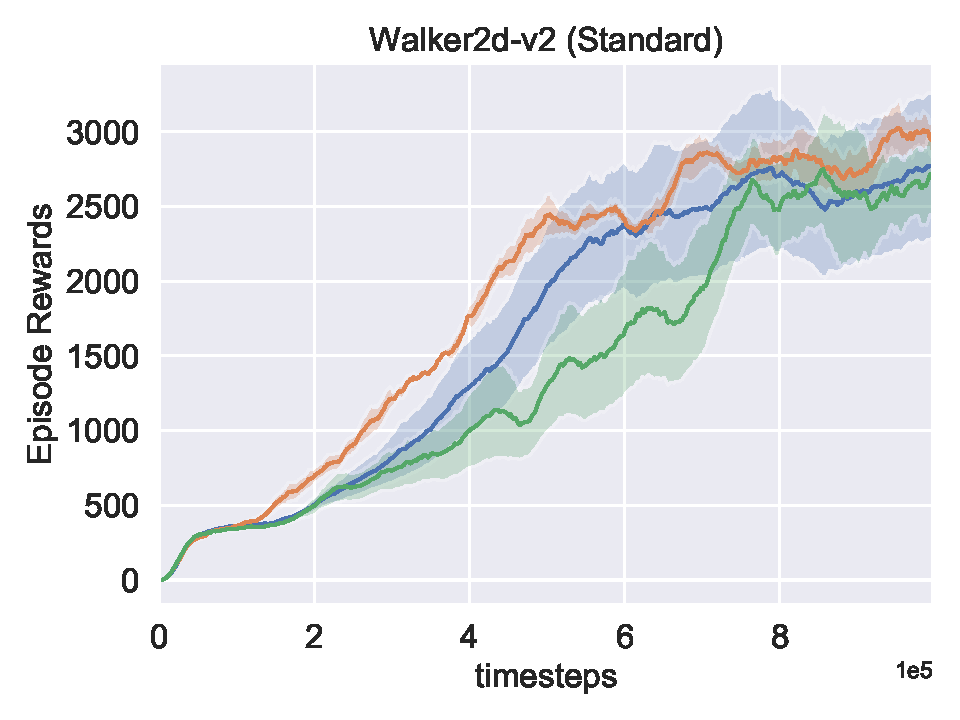
\includegraphics[width=\textwidth]{figures/chapter5/multi_frames/delay1.pdf}
    \caption{Standard}
  \end{subfigure}\hfill
  \begin{subfigure}[t]{0.49\textwidth}
    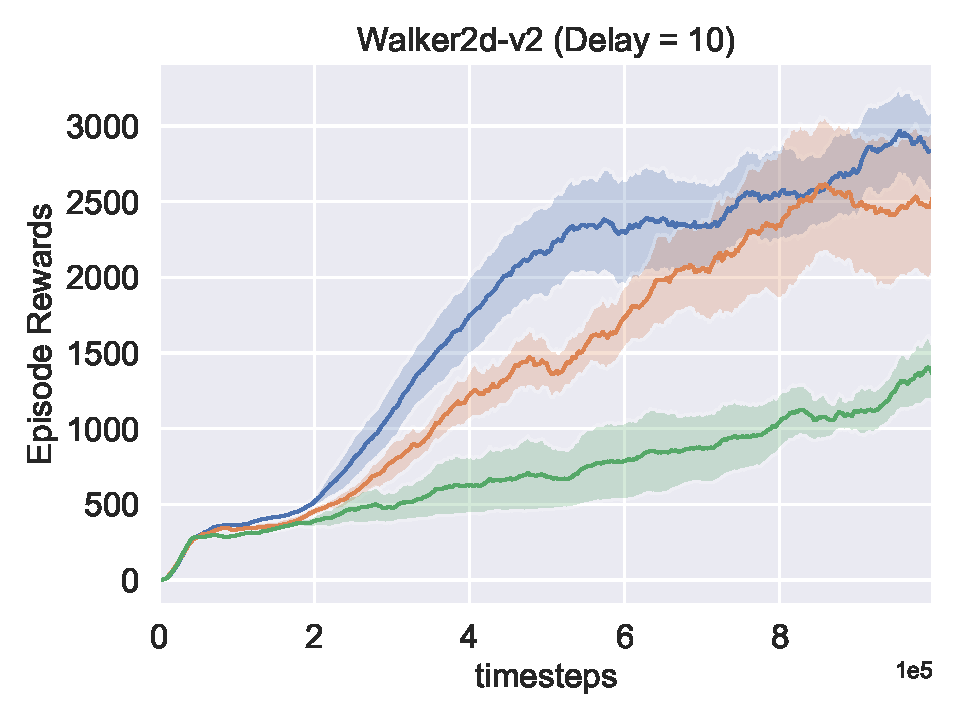
\includegraphics[width=\textwidth]{figures/chapter5/multi_frames/delay10.pdf}
    \caption{Delay=10}
  \end{subfigure}\hfill
  \begin{subfigure}[t]{0.49\textwidth}
    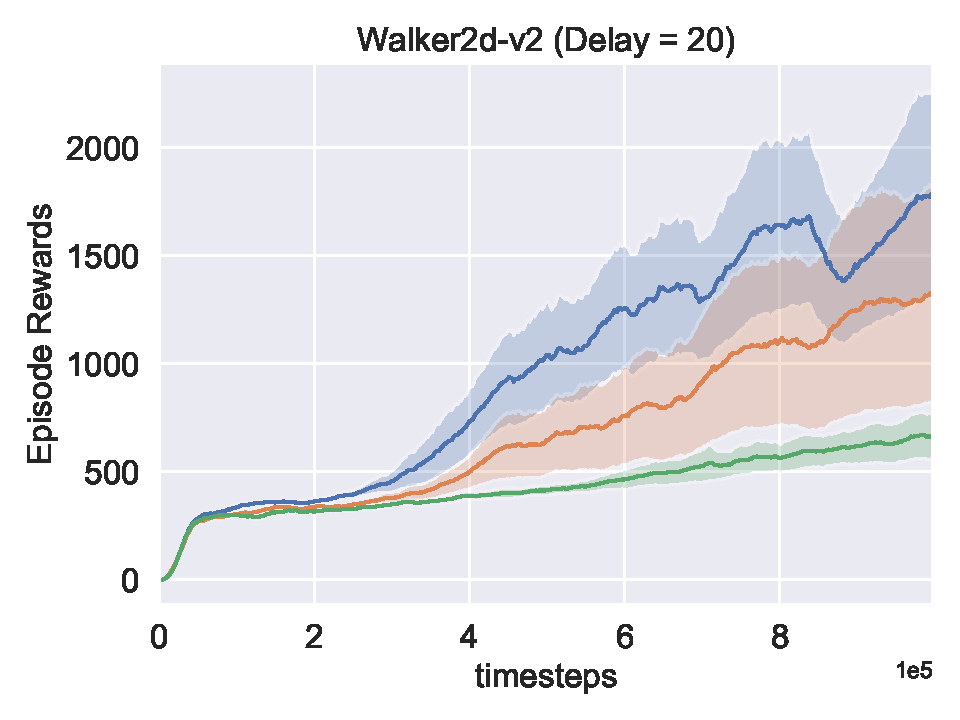
\includegraphics[width=\textwidth]{figures/chapter5/multi_frames/delay20.pdf}
    \caption{Delay=20}
  \end{subfigure}\hfill
  \begin{subfigure}[t]{0.49\textwidth}
    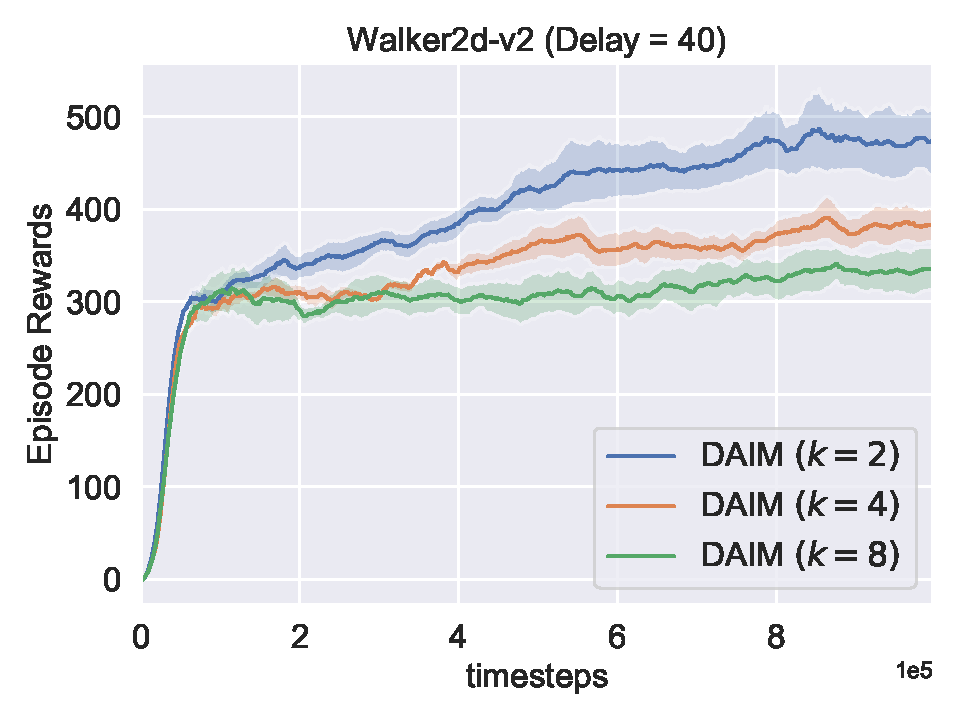
\includegraphics[width=\textwidth]{figures/chapter5/multi_frames/delay40.pdf}
    \caption{Delay=40}
  \end{subfigure}\hfill
  \caption[Results of using different length of consecutive states for calculating the intrinsic reward.]{The performance of using different size $k$ of consecutive states for calculating intrinsic rewards in the Walker2d task with standard and delayed reward settings.  The $y$-axis represents the average extrinsic rewards over the last 100 training episodes.} 
  \label{fig:multi_frames}
\end{figure}

\subsubsection{Ablation Study: Length of State Sequence}
In this section, we further investigate the performance of $\ourmethod$ using different lengths of consecutive states to calculate the intrinsic reward during training. In this case, Equation~\eqref{eq:intrinsic} can be rewritten as:
\begin{equation}
    r^{\text{in}}(s_{t:t+k-1}; \eta) = \det\left(L_{\bm{y}=\{s_{t:t+k-1}\}}\right),
\label{eq:intrinsic_multi_frame}
\end{equation}
where, $k$ is the size of consecutive states for calculating the intrinsic reward.

In Figure~\ref{fig:multi_frames}, we report on the performance of using different sizes of $k=\{2, 4, 8\}$ in calculating intrinsic rewards.  Specifically, $k=2$ represents the default setting of $\ourmethod$ which uses adjacent states for computing intrinsic rewards. From the plot, in the standard reward setting, $\ourmethod$ with different sizes $k$ achieves similar performance. In the delayed reward setting, when $k=8$, performance is worse, indicating that larger spans of consecutive states may not benefit the training. When $k=2$ or $k=4$, DAIM achieves comparable results. For Delay = 40, both $k=2$ and $k=4$ provide improvements over baselines PPO and VIME (see Figure~\ref{fig:mujoco_results}), with $k=2$ conveying the best advantage. This may be due to the fact that two adjacent states can convey information about the direction and speed of the movement; this is sufficient to convey some advantage in training. Therefore, $k=2$ was selected as the default setting for our experiments.

% \begin{figure}[t!]
%     \centering
%     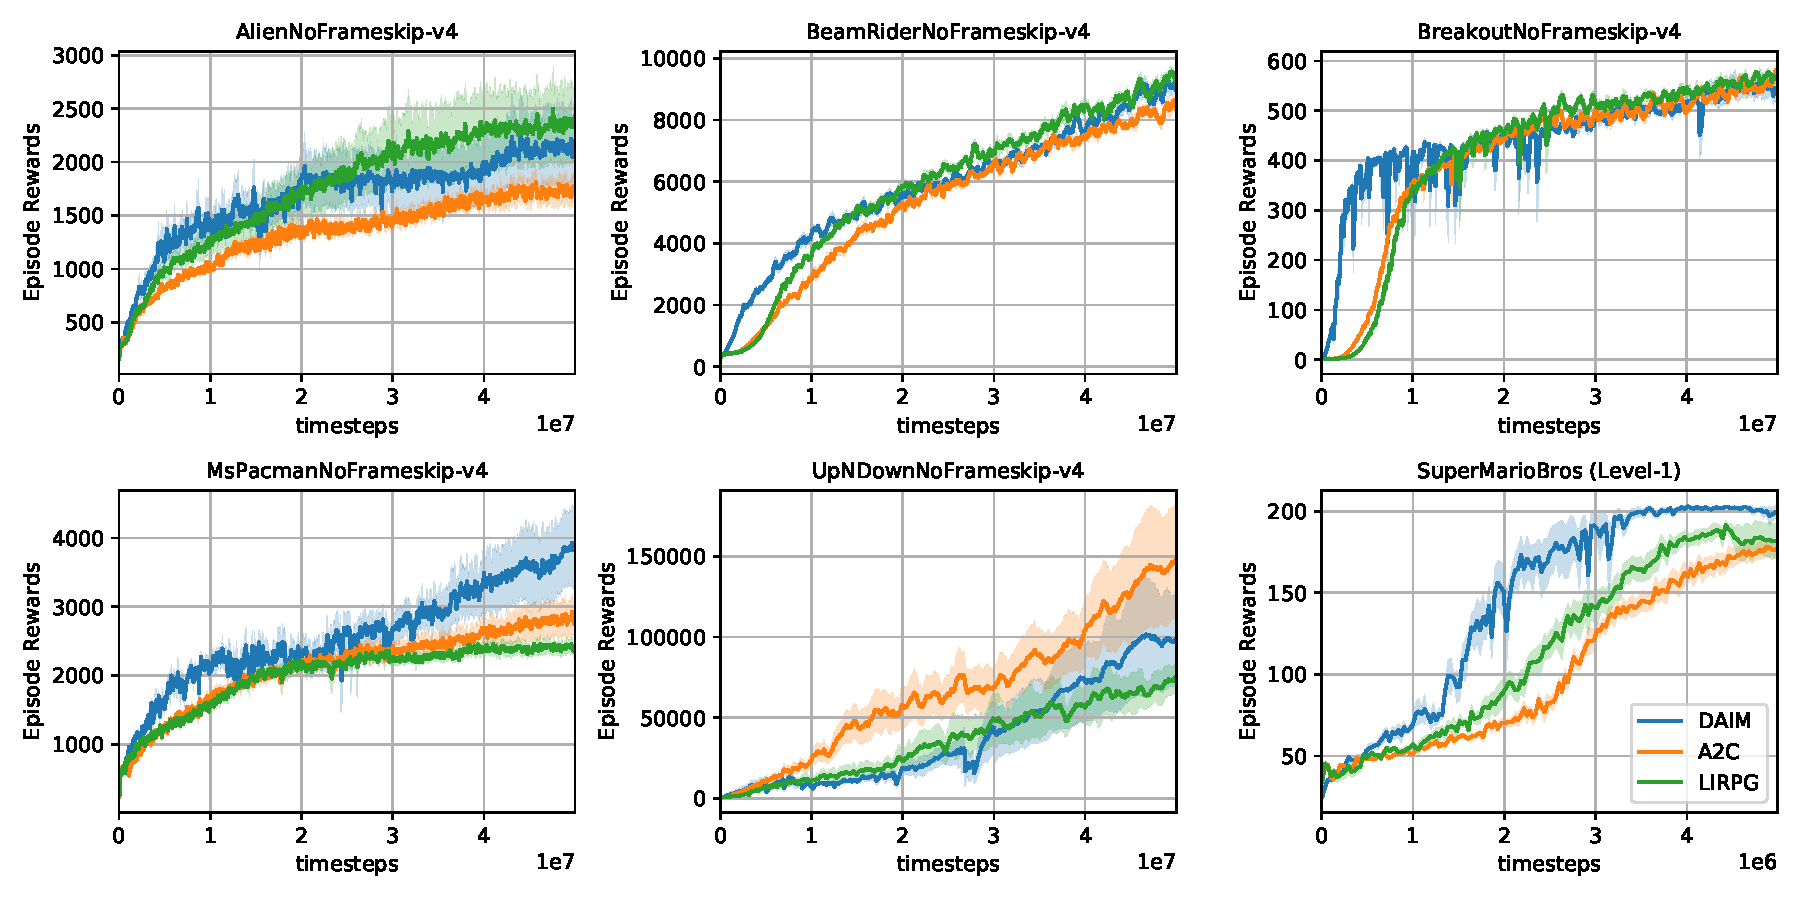
\includegraphics[width=\linewidth]{figures/chapter5/atari_mario_result.pdf}
%     \caption{Comparison between $\ourmethod$ and baseline approaches (A2C and LIRPG) in the Atari and SuperMarioBros games. The $x$-axis represents the number of timesteps in the training. The $y$-axis represents the average extrinsic rewards over the last 100  training episodes. All experiments were run using 5 different seeds. The solid lines and shaded areas in the plots represent the mean values and the standard errors, respectively, over the different seeds.}
%     \label{fig:atari_result}
% \end{figure}
\begin{figure}[h!]
\centering
  \begin{subfigure}[t]{0.49\textwidth}
    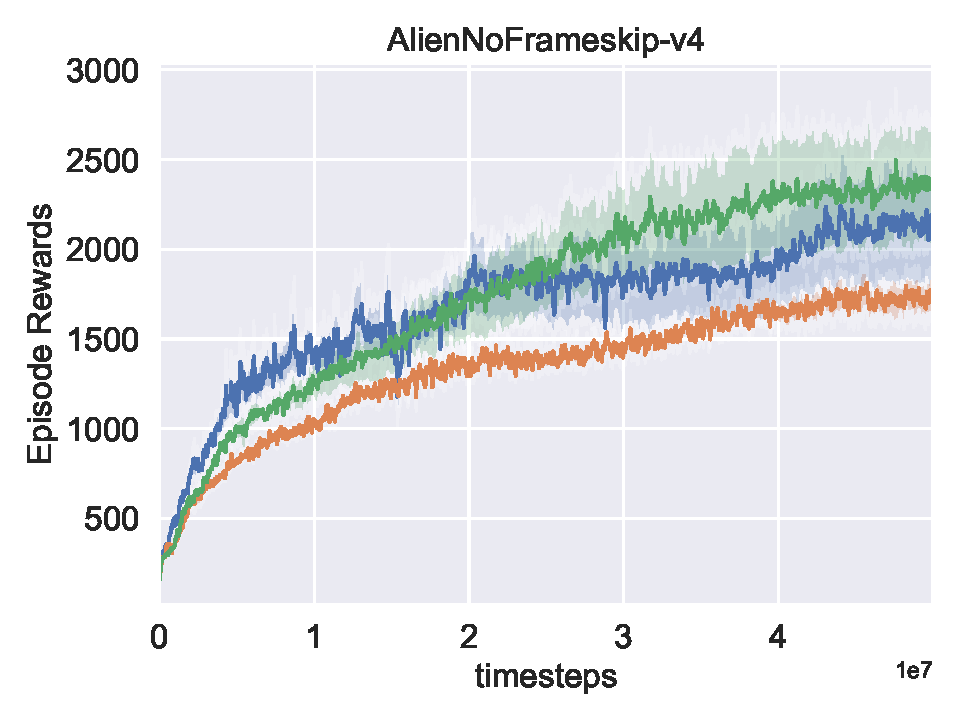
\includegraphics[width=\textwidth]{figures/chapter5/atari_exp/alien.pdf}
    \caption{Alien}
  \end{subfigure}\hfill
  \begin{subfigure}[t]{0.49\textwidth}
    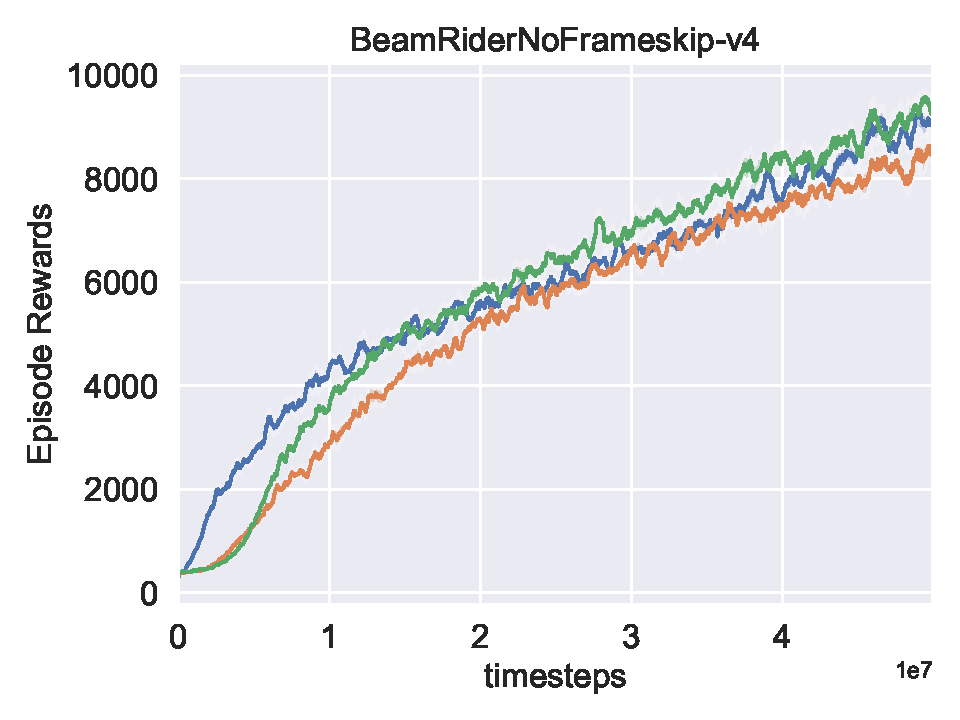
\includegraphics[width=\textwidth]{figures/chapter5/atari_exp/beamrider.pdf}
    \caption{BeamRider}
  \end{subfigure}\hfill
  \begin{subfigure}[t]{0.49\textwidth}
    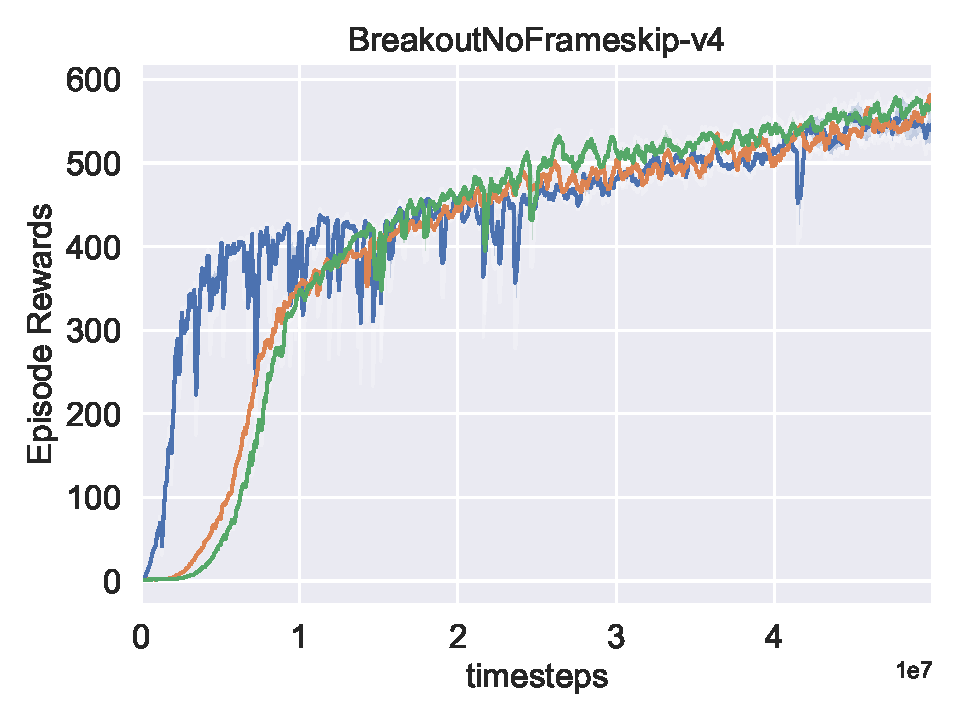
\includegraphics[width=\textwidth]{figures/chapter5/atari_exp/breakout.pdf}
    \caption{Breakout}
  \end{subfigure}\hfill
  \begin{subfigure}[t]{0.49\textwidth}
    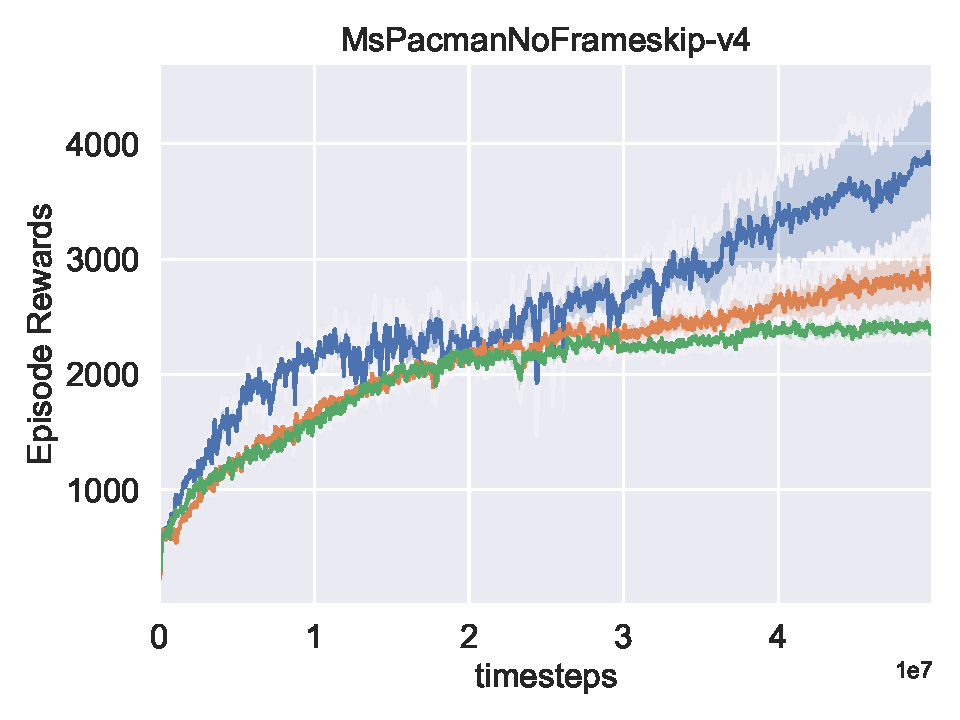
\includegraphics[width=\textwidth]{figures/chapter5/atari_exp/mspacman.pdf}
    \caption{MsPacman}
  \end{subfigure}\hfill
  \begin{subfigure}[t]{0.49\textwidth}
    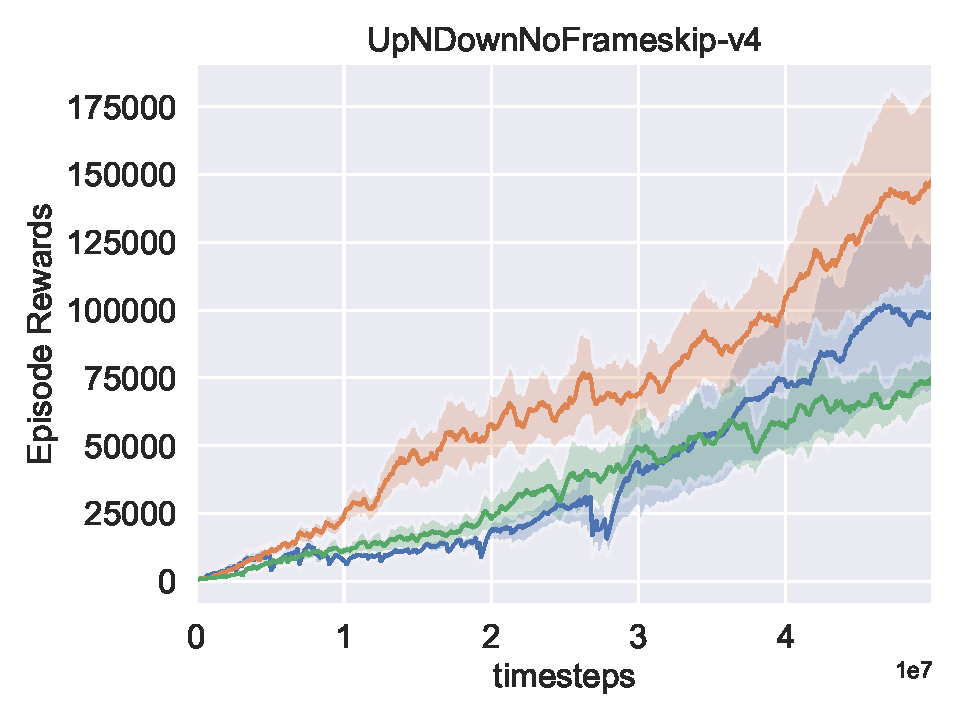
\includegraphics[width=\textwidth]{figures/chapter5/atari_exp/upndown.pdf}
    \caption{UpNDown}
  \end{subfigure}\hfill
  \begin{subfigure}[t]{0.49\textwidth}
    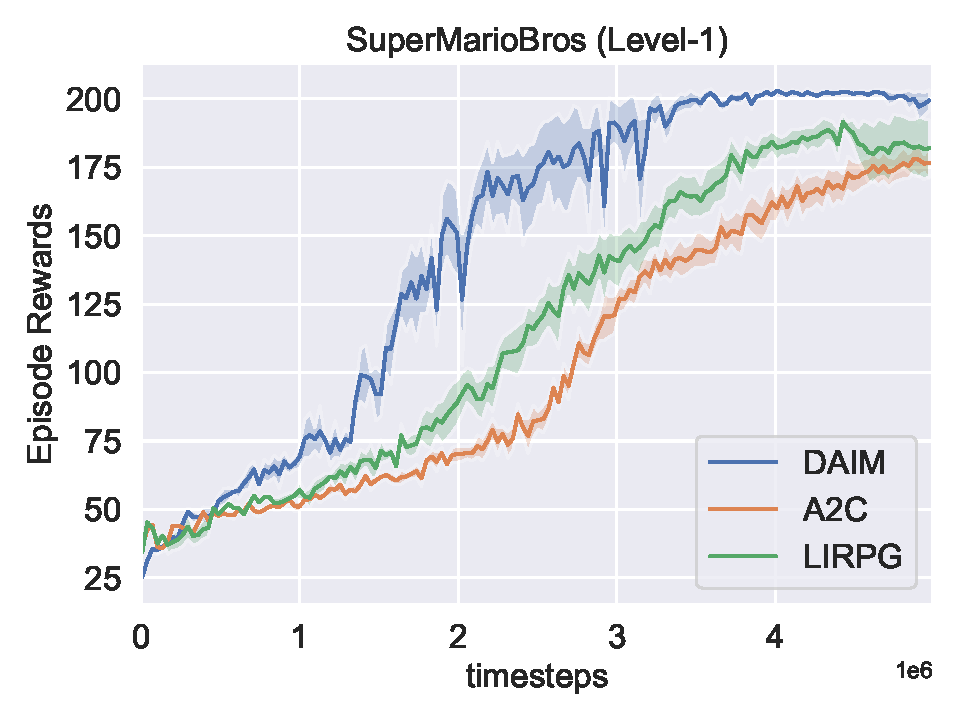
\includegraphics[width=\textwidth]{figures/chapter5/atari_exp/SuperMarioBros.pdf}
    \caption{SuperMarioBros}
  \end{subfigure}\hfill
  \caption[Results of DAIM in the arcade learning environment.]{Comparison between $\ourmethod$ and baseline approaches (A2C and LIRPG) in the Atari and SuperMarioBros games. The $x$-axis represents the number of timesteps in the training. The $y$-axis represents the average extrinsic rewards over the last 100  training episodes. All experiments were run using 5 different seeds. The solid lines and shaded areas in the plots represent the mean values and the standard errors, respectively, over the different seeds.} 
  \label{fig:atari_result}
\end{figure}


% another figure
\subsection{Results on Arcade Learning Environment}
%In both Atari games and SuperMarioBros, the hyper-parameters are set to be the same to the default A2C algorithm.

%In this experiment, Vanilla A2C and LIRPG are selected as baseline methods. For $\ourmethod$, the same CNN architecture as A2C is used upon the intrinsic module, with a 256-dimensional feature vector as output. RMSprop is selected as the optimizer with learning rate $\alpha=0.0007$. $\lambda^{\text{in}}$ and $\lambda^{\text{ex}}$ are set to 0.01 and 1 respectively. The hyper-parameters of the A2C part are kept the same to the baseline setting: number of workers is 16, timesteps per rollout of each worker are 5, entropy coefficient is 0.01, learning rate is 0.0007, discount factor $\gamma$ is 0.99, and GAE parameter $\lambda$ is 0.95. Training on the Atari games and SuperMarioBros lasts for 50 million and 5 million frames respectively. One complete training run of DAIM using one random seed takes 23.96 hours and 2.83 hours on the Atari tasks and SuperMarioBros, respectively.
Figure~\ref{fig:atari_result} and Table~\ref{tab:atari} show the performance of $\ourmethod$ against baselines. In the experiments, $\ourmethod$ has faster convergence in 5 out of 6 games (Alien, BeamRider, Breakout, MsPacman and SuperMarioBros) and achieves comparable or better results than baseline methods towards the end. In the experiments of BeamRider, Breakout, MsPacman and SuperMarioBros, $\ourmethod$ demonstrates significant improvement of learning speed in the initial stages of training. In the SuperMarioBros, $\ourmethod$ displays better performance compared to the two baseline techniques.

The explanation for the observations above is that the intrinsic rewards based on diversity can be helpful in the exploration stage of training. Thus, with the assistance of the intrinsic reward, $\ourmethod$ helps the agent explore novel states at the start of training, and achieves better or comparable performance at the end of training.

\begin{table}[h]
    \centering
\resizebox{\textwidth}{!}{
    \begin{tabular}{c|cccccc}
    \toprule
        Methods & Alien & BeamRider & Breakout & MsPacman & UpNDown & SuperMarioBro \\
        \midrule
         A2C & 1698$\pm$129 & 8380$\pm$205& \textbf{567$\pm$10} & 2739$\pm$221 & \textbf{147069$\pm$3923} & 175$\pm$6\\
         LIRPG & \textbf{2429$\pm$379} & \textbf{9183$\pm$205} & \underline{566$\pm$8} & \underline{2405$\pm$77} & 75088$\pm$9299 & \underline{182$\pm$10}\\
         \midrule
         DAIM & \underline{2132$\pm$341} & \underline{9001$\pm$131} & 544$\pm$23 & \textbf{3874$\pm$542} & \underline{98683$\pm$28430} & \textbf{198$\pm$4}\\
         \bottomrule
    \end{tabular}
    }
    \caption[Average reward of DAIM in the arcade learning environment in the final epoch during training.]{Quantitative results comparison between DAIM and other baseline methods (A2C and LIRPG) in the Atari and SuperMarioBro games. In the table, it shows final average extrinsic rewards $\pm$ standard error across 5 different seeds of last 100 episodes in the training. The best and the second best results are (\textbf{bold}) and (\underline{underline}), respectively.}
    \label{tab:atari}
\end{table}

\section{Discussion}
\begin{table}[h!]
    \centering
    \resizebox{0.7\textwidth}{!}{
    \begin{tabular}{c|c|c|c|c}
    \toprule
           & PPO~\cite{schulman2017proximal} & LIRPG~\cite{zheng2018learning} & VIME~\cite{NIPS2016_abd81528} & DAIM\\
        \midrule
        Time  & 00:28:50 & 1:23:43 & 03:18:36 & 01:26:21 \\
        \bottomrule
    \end{tabular}
    }
    \vspace{0.2em}
    \caption[Training time comparison between DAIM and other baselines.]{Training time (hours:minutes:seconds) of DAIM and baseline approaches on the MuJoCo tasks.}
    \label{tab:time_daim}
\end{table}

In this chapter, the DPPs framework is employed to measure the diversity of state sequences; it is shown this can be used to create an intrinsic reward that encourages state-space exploration in on-policy learning; we term this variant diversity-augmented intrinsic motivation (DAIM). The update of the proposed intrinsic reward module is formulated as a bi-level optimisation problem. During training, as the agent tries to maximise mixture returns, the bi-level optimisation guarantees that extrinsic returns are also maximised. Based on the extensive experiments, DAIM achieves improvements in continuous control in delayed-reward problems when compared to well-known on-policy training approaches of similar complexity, such as LIRPG~\cite{zheng2018learning} and VIME~\cite{NIPS2016_abd81528}. Table~\ref{tab:time_daim} displays the training time of DAIM and other baselines on one MuJoCo task with a single random seed. From the table, DAIM requires longer training time than the vanilla PPO because of its bi-level optimisation steps. However, DAIM and other extension algorithms for PPO have similar training time, such as LIRPG and VIME. DAIM also accelerates the convergence of training agents on ALE compared to the baseline training approaches. In the work of this chapter, DAIM is combined with PPO and A2C; in principle, DAIM could also be applied to other on-policy RL algorithms, such as TRPO~\cite{schulman2015trust} or SVPG~\cite{liu2017stein}. 

The wider implications of these experiments should be assessed against off-policy training approaches, e.g., the DQN~\cite{mnih2015human} for discrete control or DDPG~\cite{lillicrap2015continuous} for continuous control, which are considered more sample efficient than on-policy approaches. The advantage of on-policy RL algorithms is generally that they are more stable in training and are more robust to hyperparameter settings.

In the future, we will investigate how to extend the DAIM approach to off-policy sampling and address more challenging tasks, such as Montezuma's Revenge. Furthermore, we can also combine the self-imitation learning loss in Chapter~\ref{ch:esil} with the diversity-based intrinsic rewards to achieve a further improvement in tasks with a sparse reward setting.
%with even sparser reward structure